\chapter{Results}

\begin{figure}[H]
    \centering
    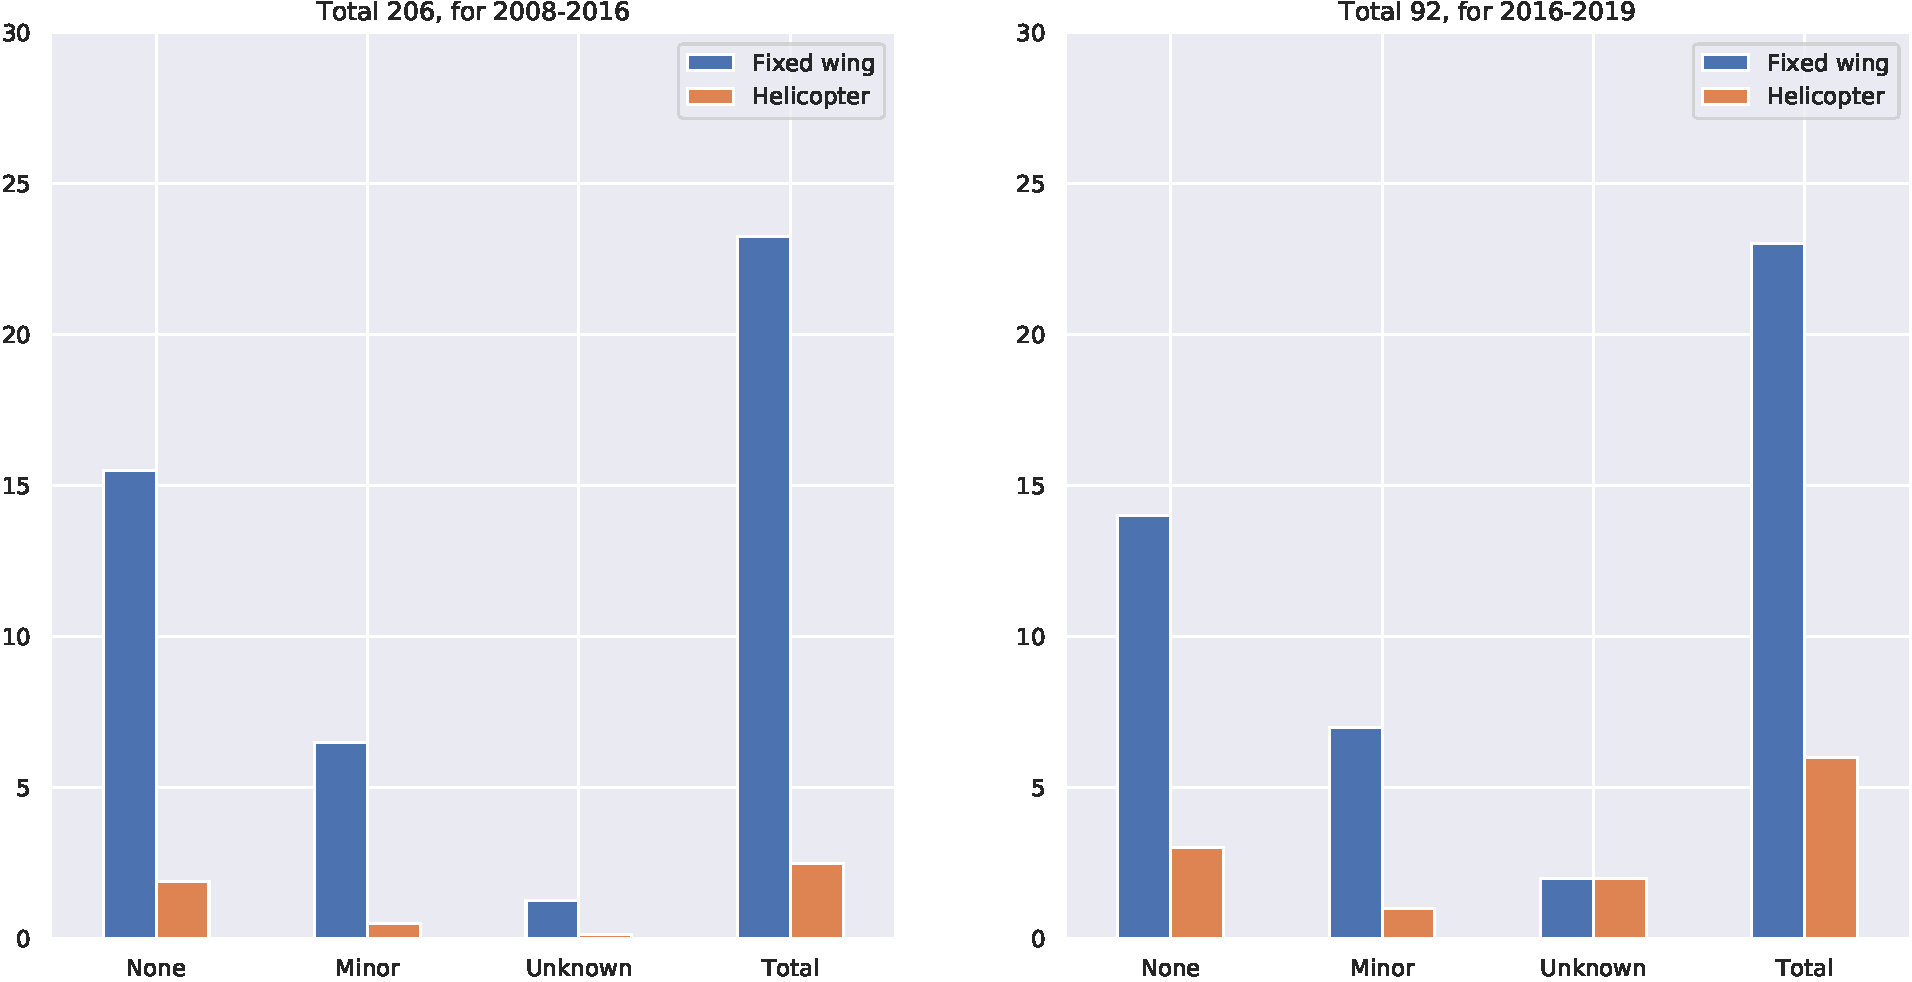
\includegraphics[width=\textwidth]{Figures/Casesperyear.pdf}
    \caption{}
    \label{fig:casesperyear}
\end{figure}

\section{}
To verify the skill of the \acrshort{hti}, the index has been divided into sub-indices as described in Section \ref{sec:decomposition}. The helicopter cases happening after the operational forecast was introduced have their indices plotted in Figure \ref{fig:HeliAccum}. The figure shows that for all the eleven cases the \acrshort{hti}-value is atleast .50. If one also takes into account each sub-indices contribution as plotted in Figure \ref{fig:HeliDecomp}, one can see that the temperature parameter has it's full value for all cases, whilst the third case has a value of  $\sim .57/4$ due to the interpolated temperature from the model was found to be  $\sim -.57 ^{\circ}C$
The total "correctly" forecast cases for different thresholds is shown in Table \ref{tab:HeliCont}. 

\section{Discussion to last sec}
As discussed in Section \ref{ch:background}, the limit for precipitation was chosen to reduce the wrongly identified cases. Instead the upper limit of precipitation should be higher, and the area around looking for precipitation should be increased (Maybe to decrease error due to model dryness as discussed in model)

https://www.energyvoice.com/other-news/102241/lighting-strike-forces-north-sea-helicopter-to-make-emergency-landing/
https://draugen.industriminne.no/nb/2018/05/25/helikopter-truffet-av-lyn/#footnote_target_1
https://www.brunsvika.net/nyhetsarkiv-alle-artikler/2009/4077-lynnedslag-i-helikopter
https://assets.publishing.service.gov.uk/media/54230184e5274a1317000b3d/dft_avsafety_pdf_501972.pdf

\begin{table}[H] 
    \centering
    \begin{tabular}{c|c|c|c}
        Forecast & With Accumulated & Without Accumulated & Missed \\ \hline
        >Yellow (0.73) & 9 & 7 & 2\\
        >Orange (0.90) & 2 & 2 & 7\\ 
        >Red (0.99) & 0 & 0 & 11\\
    \end{tabular}
    \caption{Contingency table based on the $11$ Helicopter cases in Figure \ref{fig:HeliAccum}}
    \label{tab:HeliCont}
\end{table}

\begin{table}[H]
    \centering
    \begin{tabular}{c|c|c|c}
        Forecast & With Accumulated & Without Accumulated & Missed \\ \hline
        >Yellow (0.73) & 22 & 21 & 14\\
        >Orange (0.90) & 10& 8& 25\\ 
        >Red (0.99) & 4& 3& 30\\
    \end{tabular}
    \caption{Contingency table based on the $34$ Fixed wing cases in Figure \ref{fig:FWAccum}}
    \label{tab:FWCont}
\end{table}


\begin{figure}[H]
    \centering
    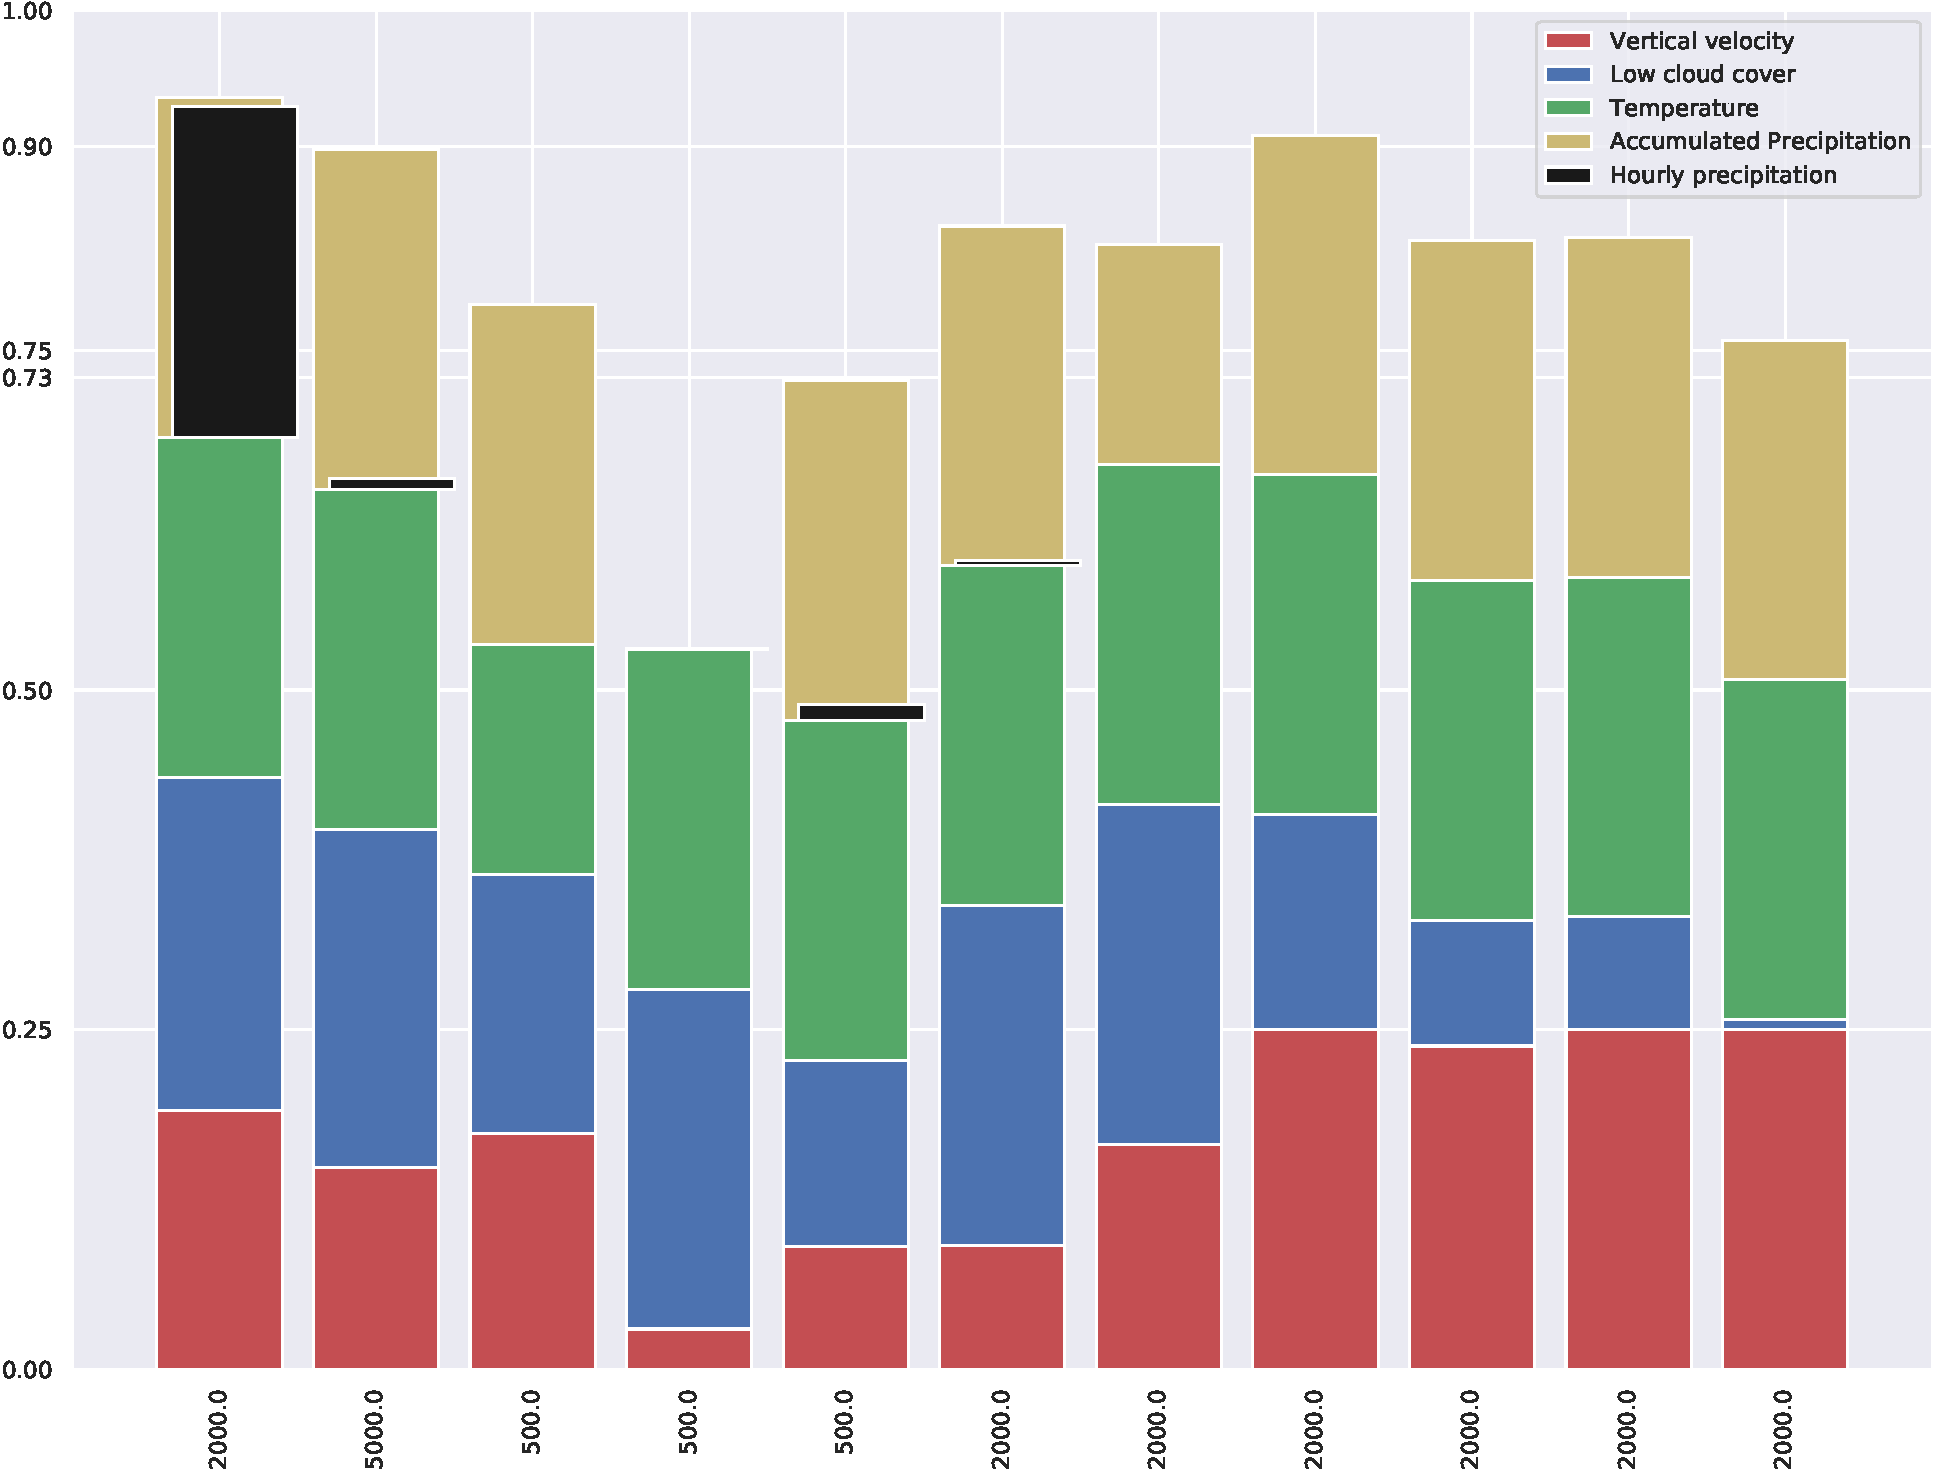
\includegraphics[width=\textwidth]{Figures/HeliAccum.pdf}
    \caption{Contributions from the different sub-indices, for Helicopter cases during the operational forecast. Black on yellow is correction made by using the hourly precipitation instead of accumulated precipitation.}
    \label{fig:HeliAccum}
\end{figure}

\begin{figure}[H]
    \centering
    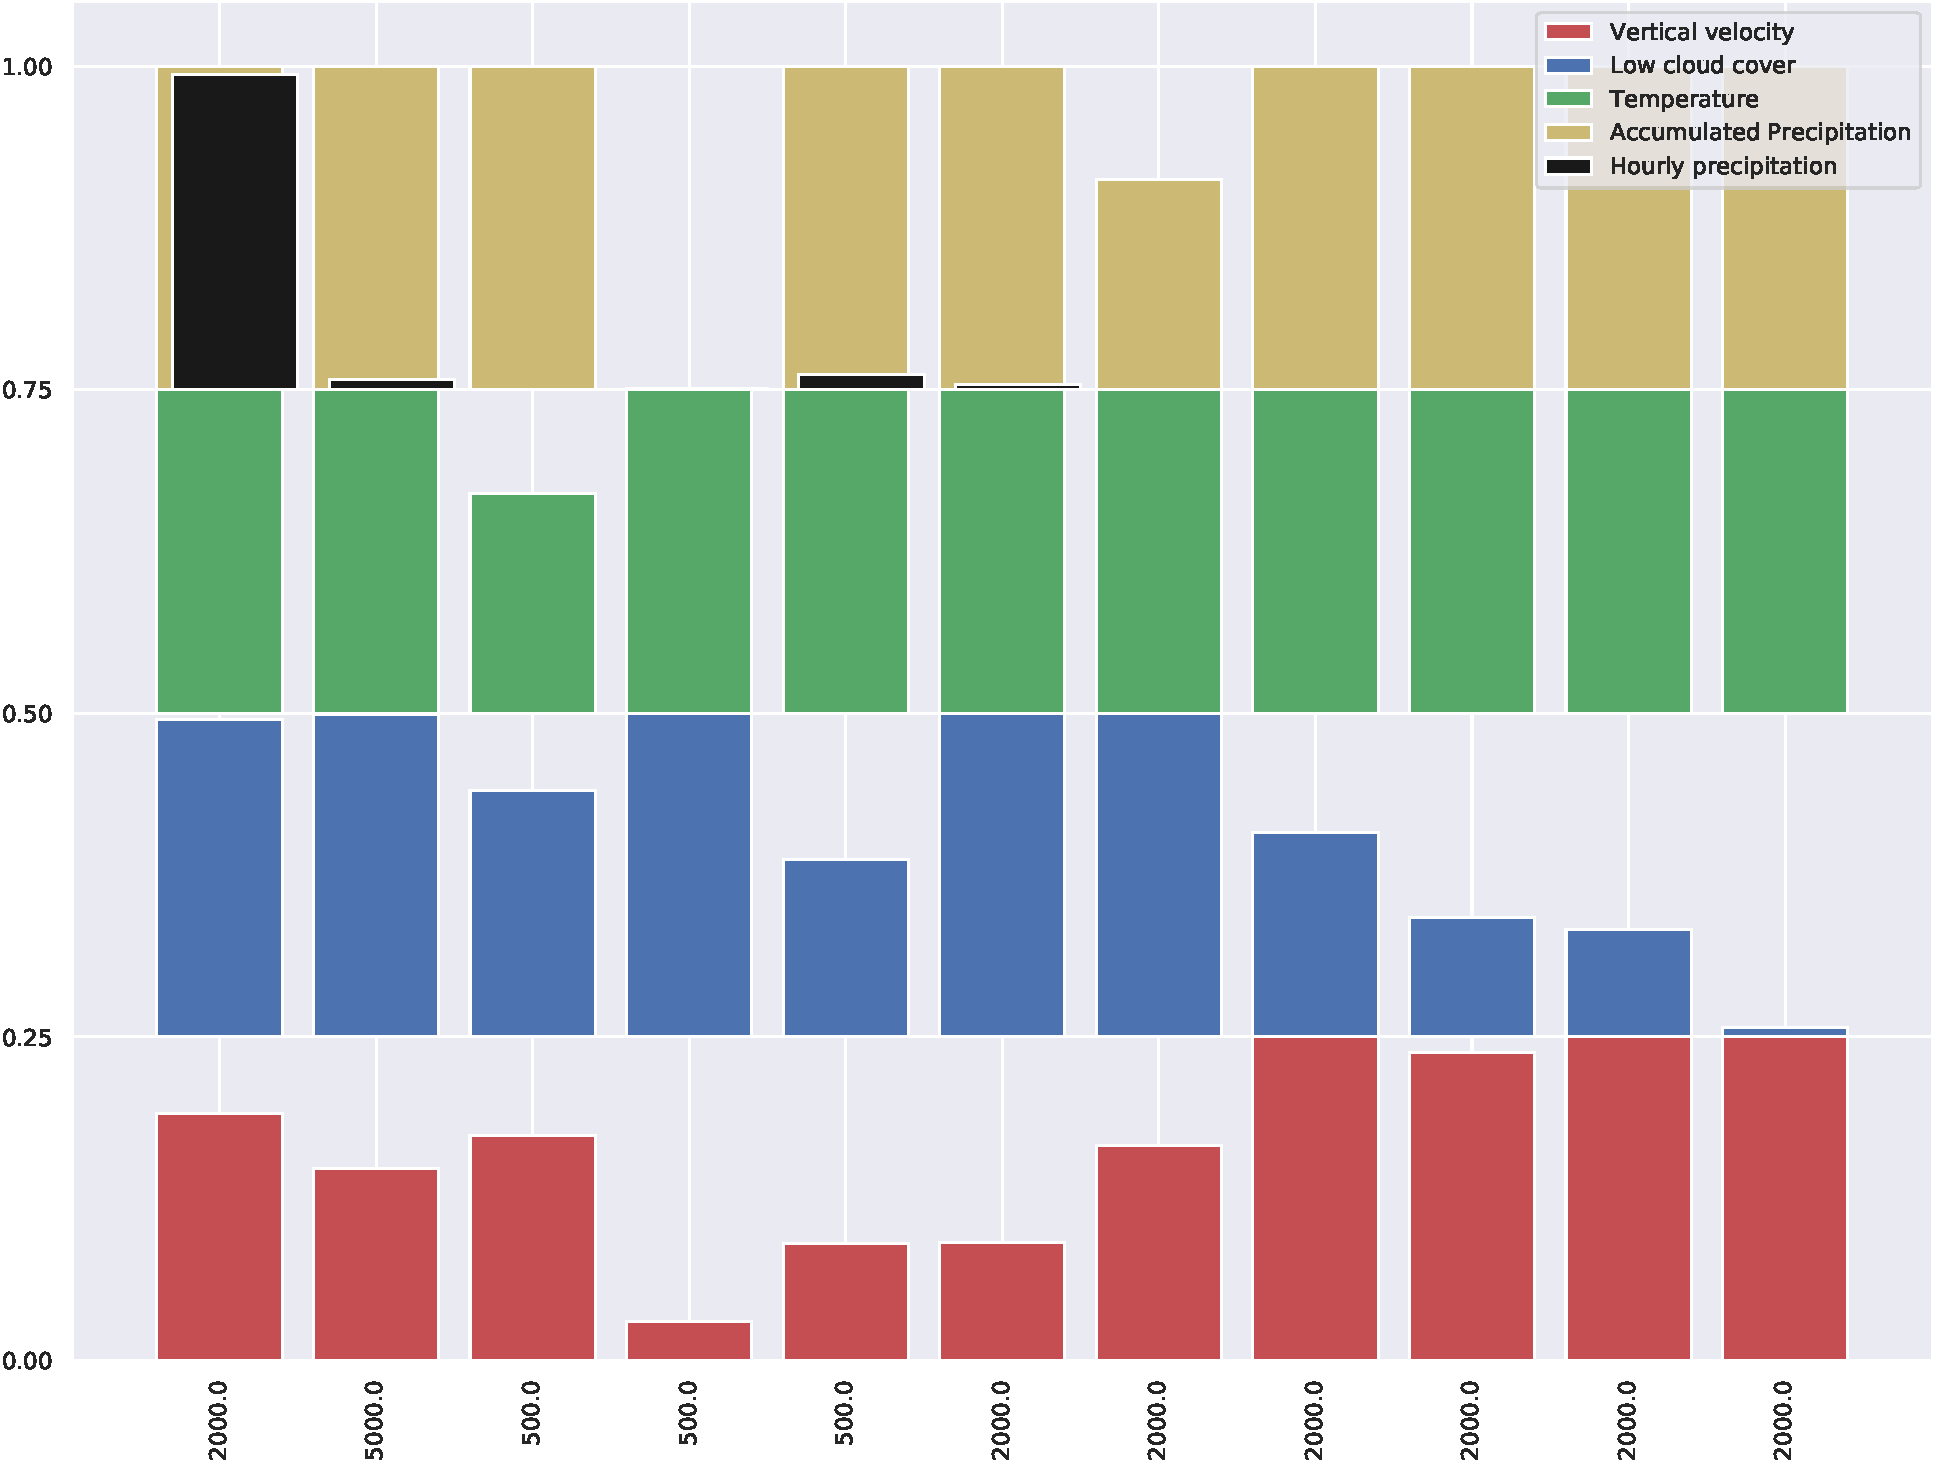
\includegraphics[width=\textwidth]{Figures/HeliDecomp.pdf}
    \caption{Same as \ref{fig:HeliAccum}, but clearly delineated between the sub-indices}
    \label{fig:HeliDecomp}
\end{figure}

\begin{figure}[H]
    \centering
    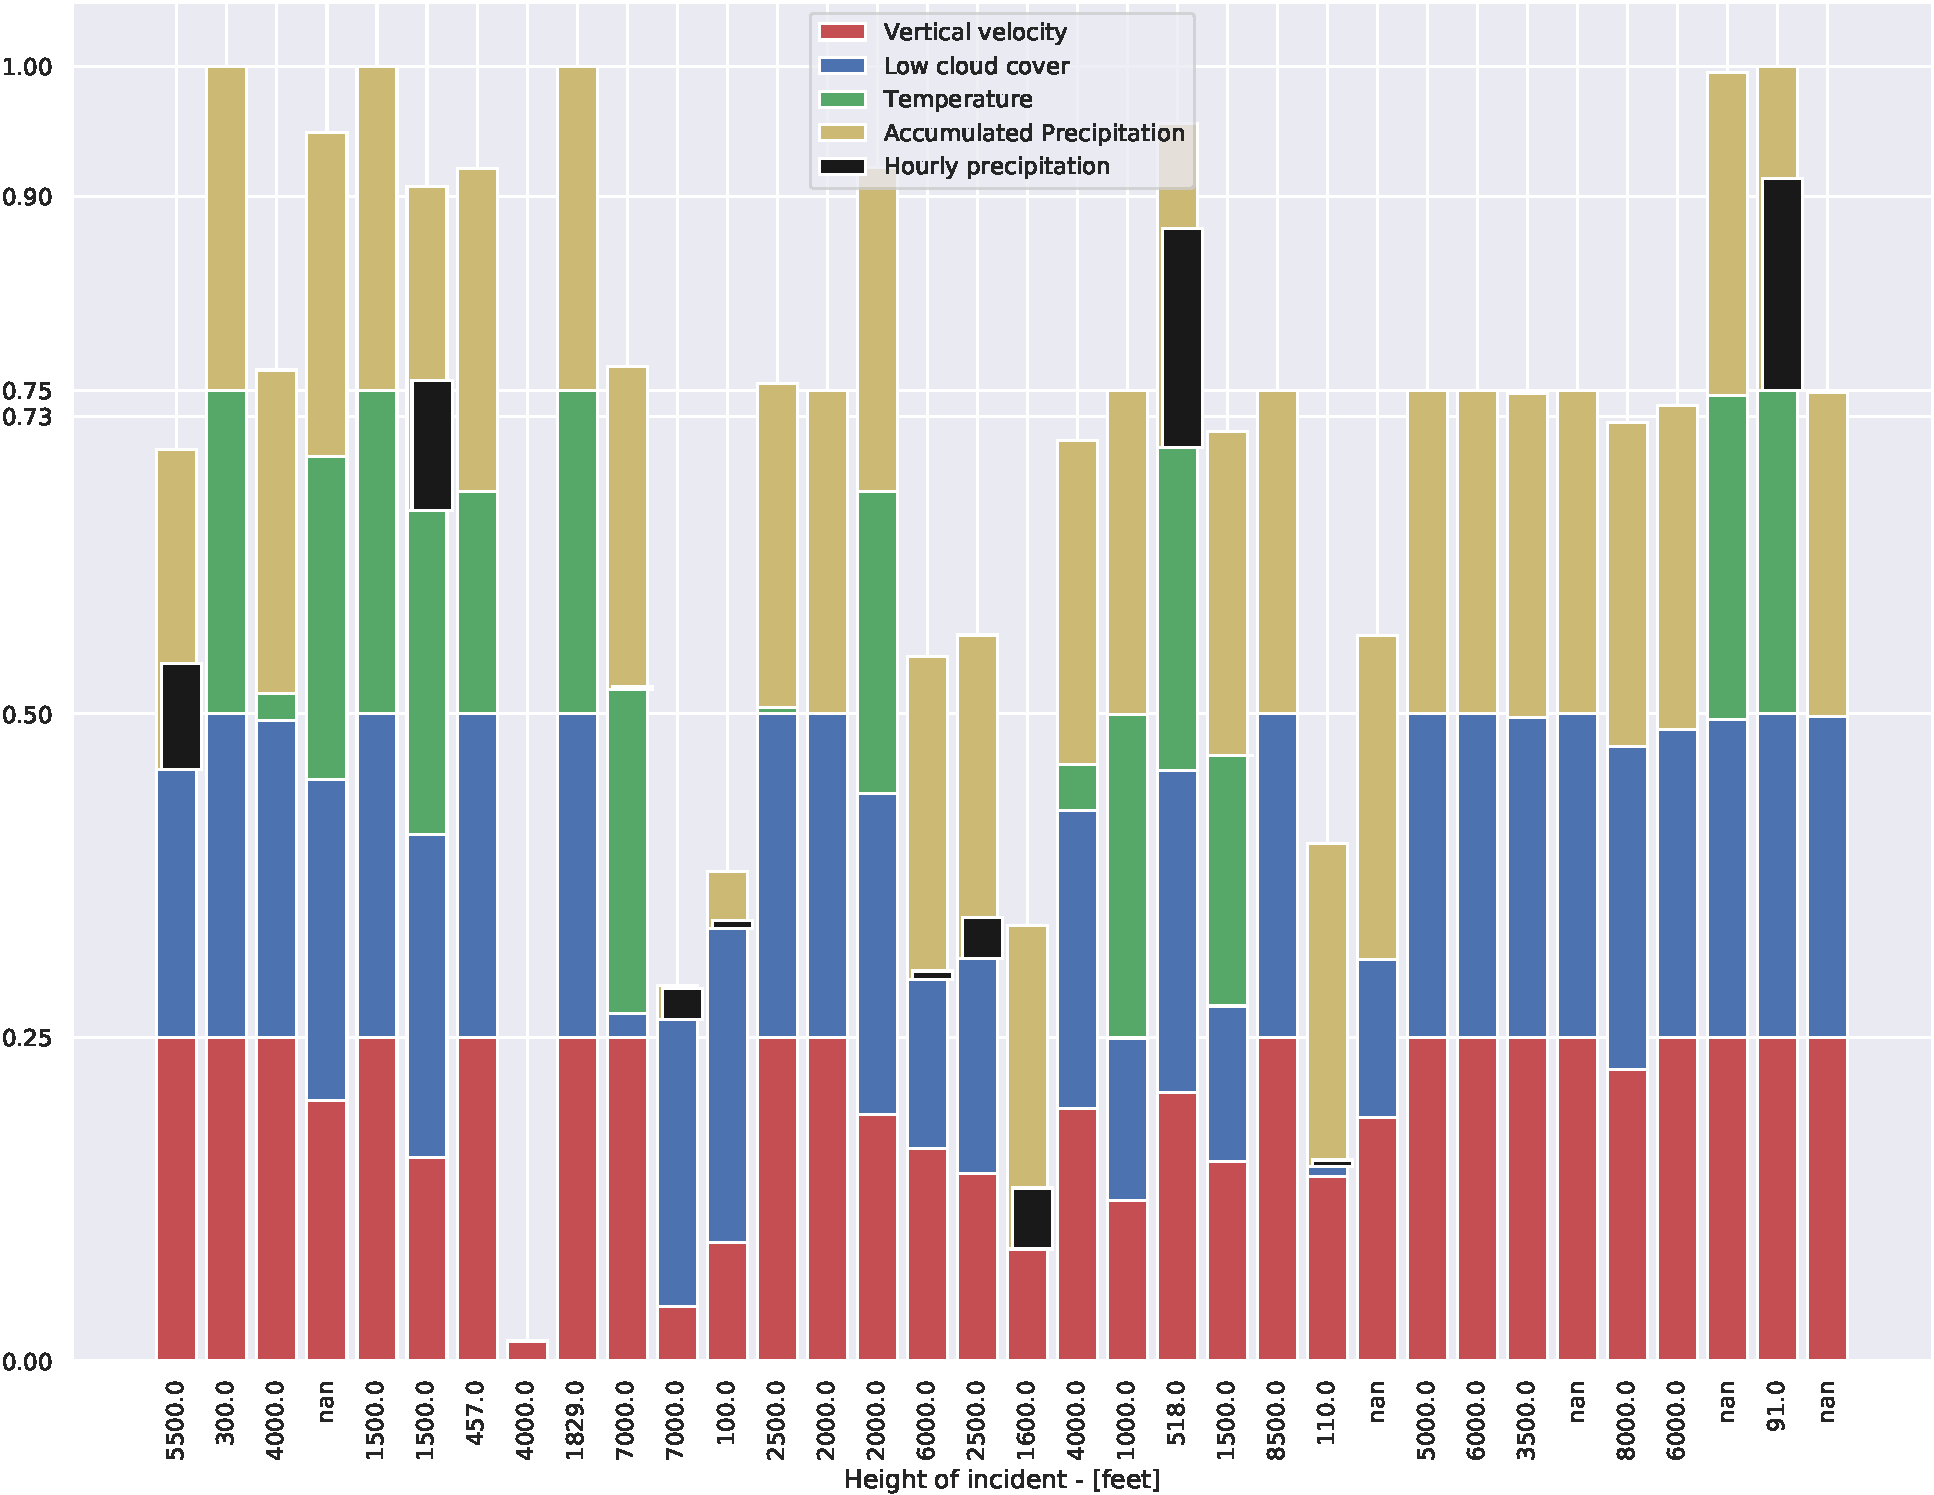
\includegraphics[width=\textwidth]{Figures/FWAccum.pdf}
    \caption{Contributions from the different sub-indices, for Fixed wing cases during the operational forecast. Black on yellow is correction made by using the hourly precipitation instead of accumulated precipitation.}
    \label{fig:FWAccum}
\end{figure}

\begin{figure}[H]
    \centering
    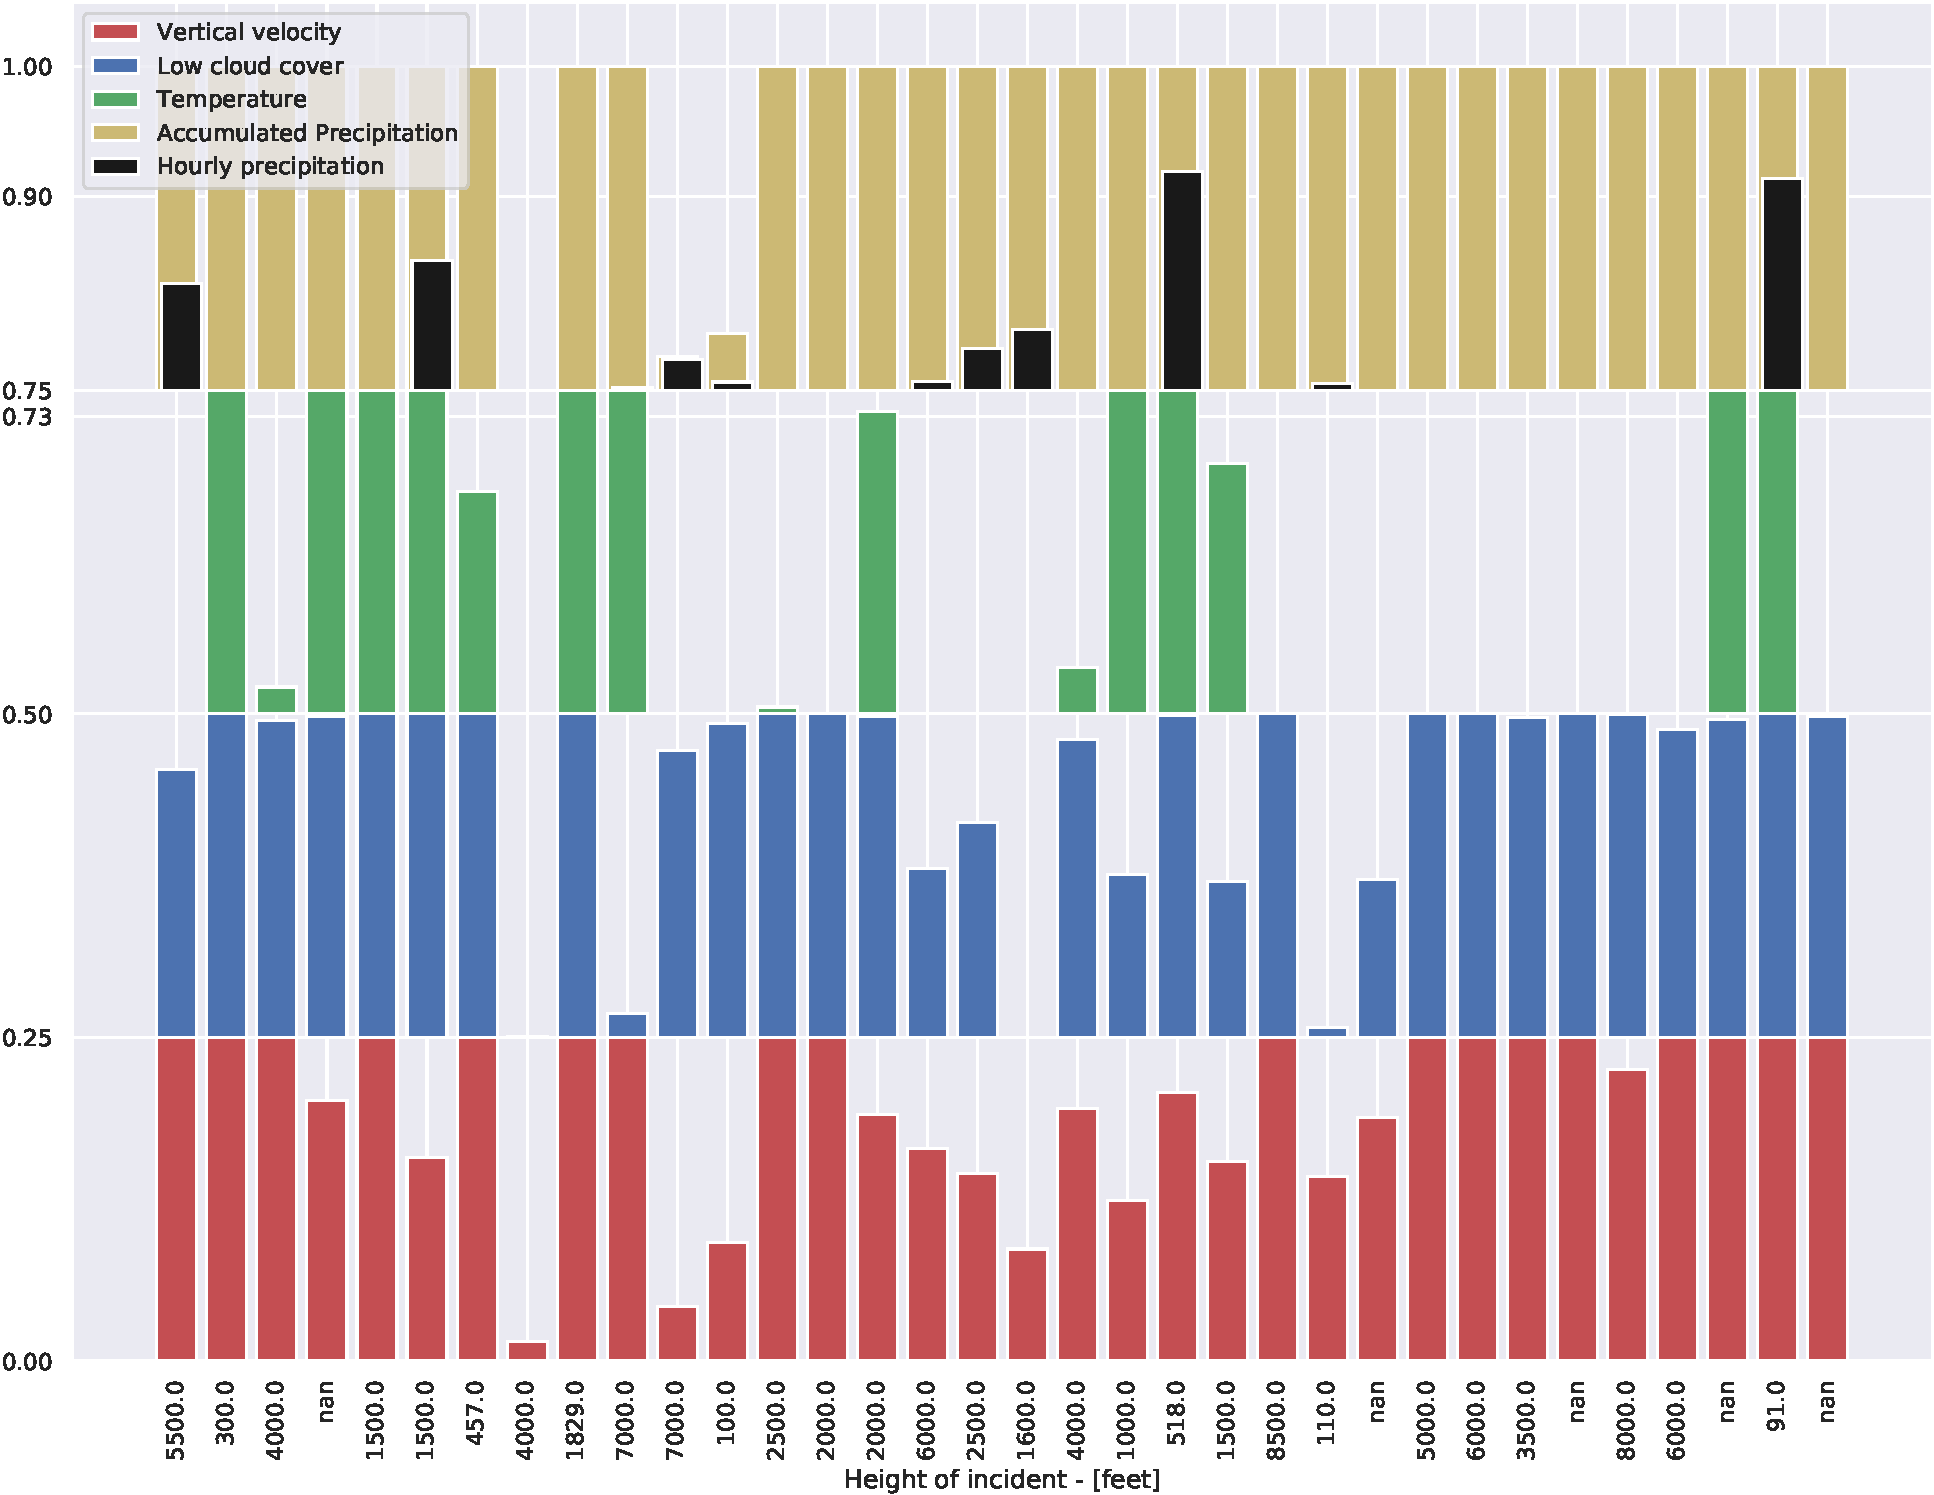
\includegraphics[width=\textwidth]{Figures/FWDecomp.pdf}
    \caption{Same as \ref{fig:FWAccum}, but clearly delineated between the sub-indices}
    \label{fig:FWDecomp}
\end{figure}





To prevent cases from differing climatic regions from interfering with each other, the cases are divided into climatic zones, as shown in Figure \ref{fig:Stationsmap}. These zones are chosen to give approximately equal climates, and such that the amount of cases are equal for the zones. The amount per zones are shown in Figure \ref{fig:soner}.

\begin{sidewaysfigure}
    \centering
    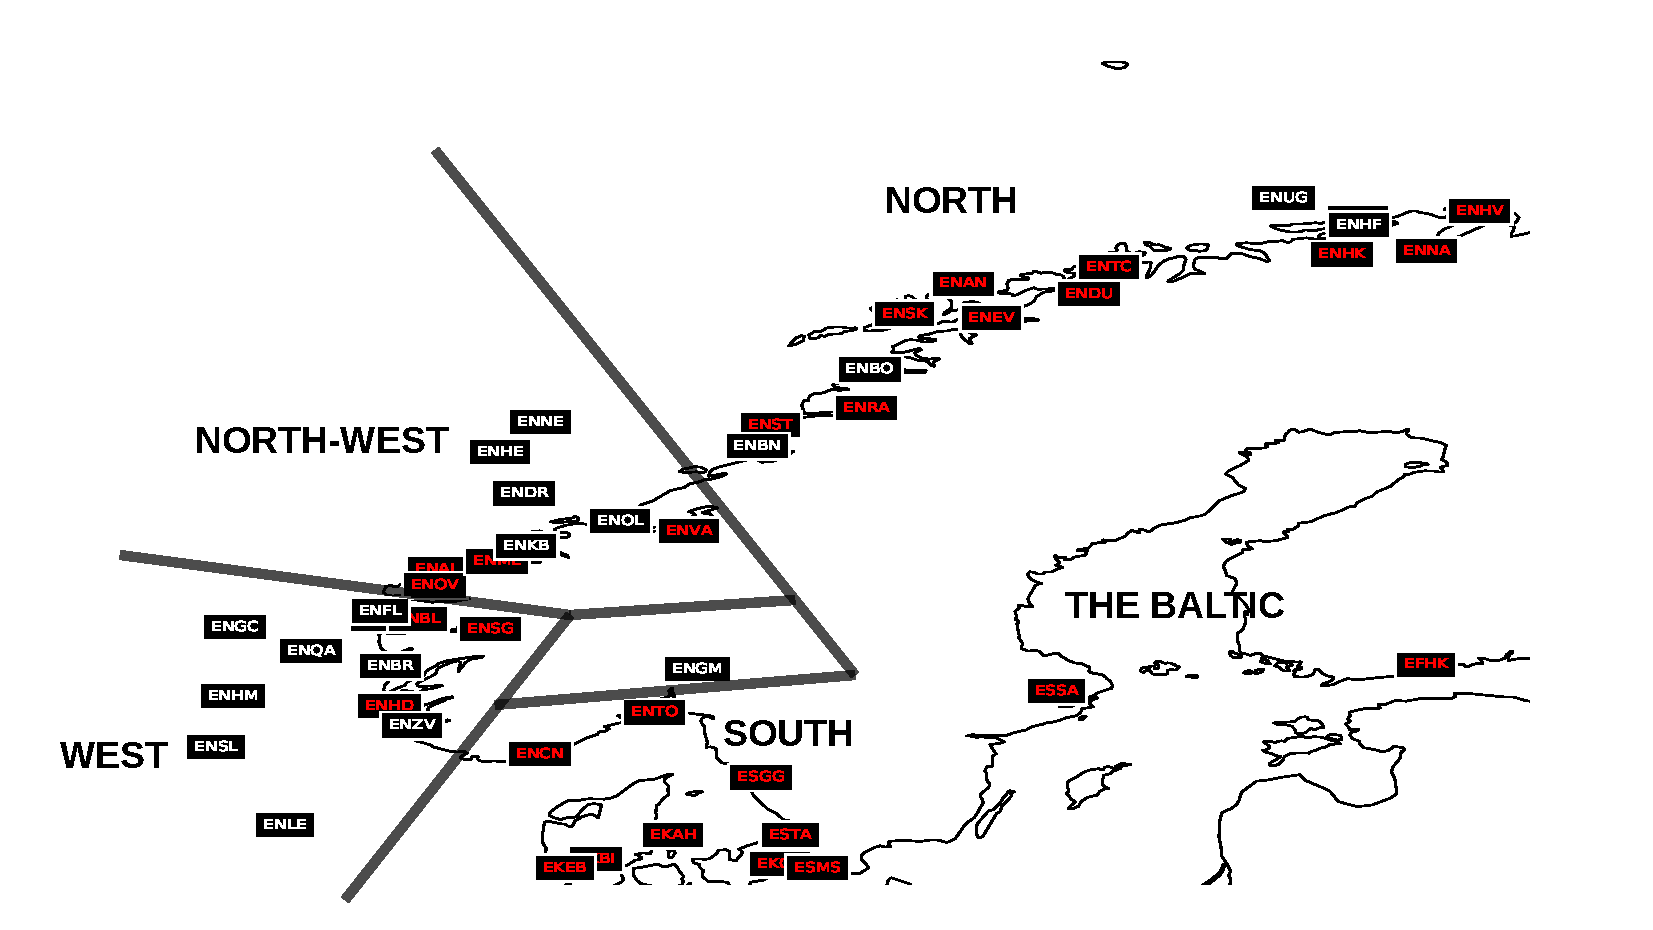
\includegraphics[width=\textwidth]{Figures/METARandHIT.pdf}
    \caption{Zones used in this thesis, with METAR-stations in white, and unique places with incidents in red.}
    \label{fig:Stationsmap}
\end{sidewaysfigure}

\section{Analysis of the AVINOR lightning dataset}
\begin{figure}
    \centering
    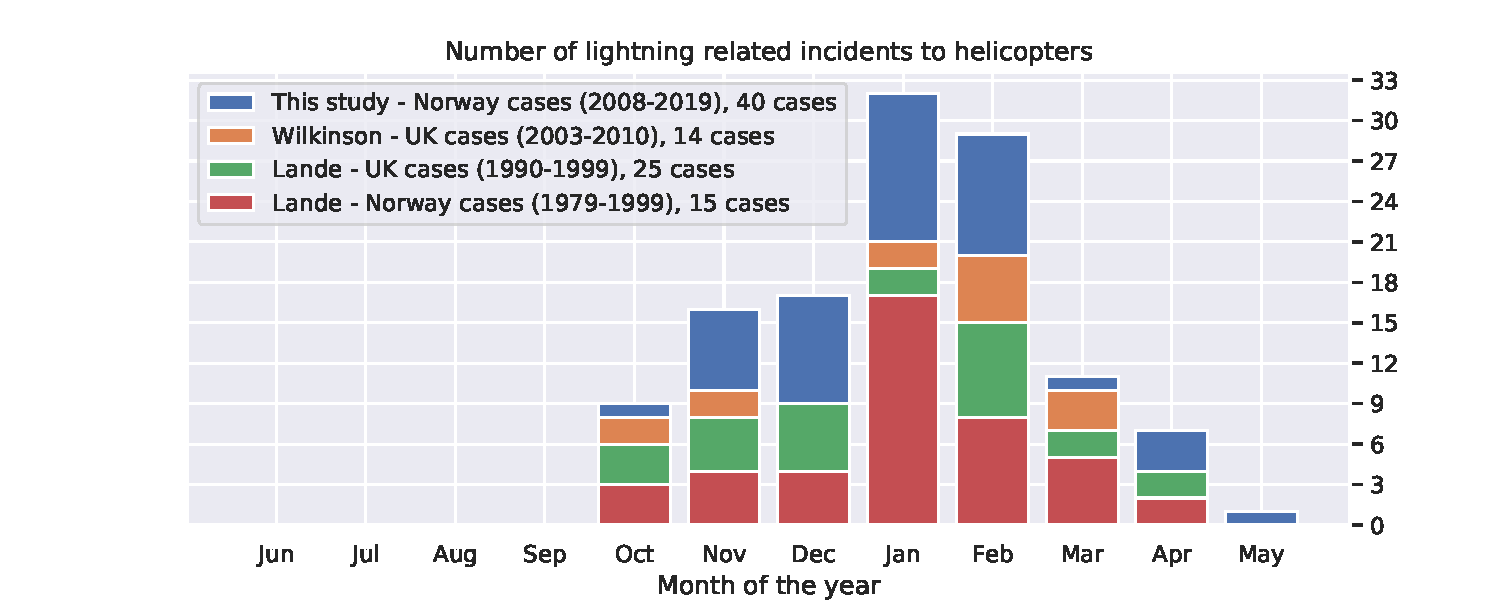
\includegraphics[width=\textwidth]{Figures/yearlydistribution.pdf}
    \caption{Seasonal variation of helicopter cases, showing no cases in June to September. Same as Figure \ref{fig:landewilk}, with cases looked at in this study added to it. Older data is produced from \cite{lande1999} and \cite{wilkinson2013}. Legend notes time-periods and amount of cases in each study. }
    \label{fig:yearlyvariation}
\end{figure}

As one can see from Figure \ref{fig:yearlyvariation}, the helicopter cases added in this study have the same seasonal variation as in earlier \acrshort{htl} studies (\cite{wilkinson2013}, \cite{lande1999}). Although this novel data set has one case in May, this may be attributed to the Norwegian climate being colder than the United Kingdom's and can be looked at as a statistical anomaly. Note that the peak of \acrlong{htl} is in the mid-winter (January, February). 

Looking at the whole dataset as in Figure \ref{fig:helivsfw}, we see that helicopter cases are distributed as described earlier but the \acrshort{fwtl} cases are distributed evenly throughout the year with a peak in the late Norwegian summer (August), mid-spring (April) and early-to-mid winter (December-January). To explain the peak in April, we will need to study the geographical variations  in helicopter cases as plotted in Figure \ref{fig:helisoner}. Here we see that the three helicopter cases in April are only on the north coast. These may be attributed to a climatological shift, north coast April being relatively comparable to west coast February. The peak in August may be attributed to this being the most active month of lightning activity as late summer is climatologically warmer, so more convection happens in general. Looking at the \acrshort{fwtl} instead (Figure \ref{fig:soner}), we see that April has more cases in the southern zone.

Continuing with Figure \ref{fig:soner}, we see that the cases have their peak for the West, North West and North coast in the winter months, while the Southern Baltic zone and Gardemoen have their peak during the summer months. This hints at a climatological difference between these zone groups.

\begin{figure}
    \centering
    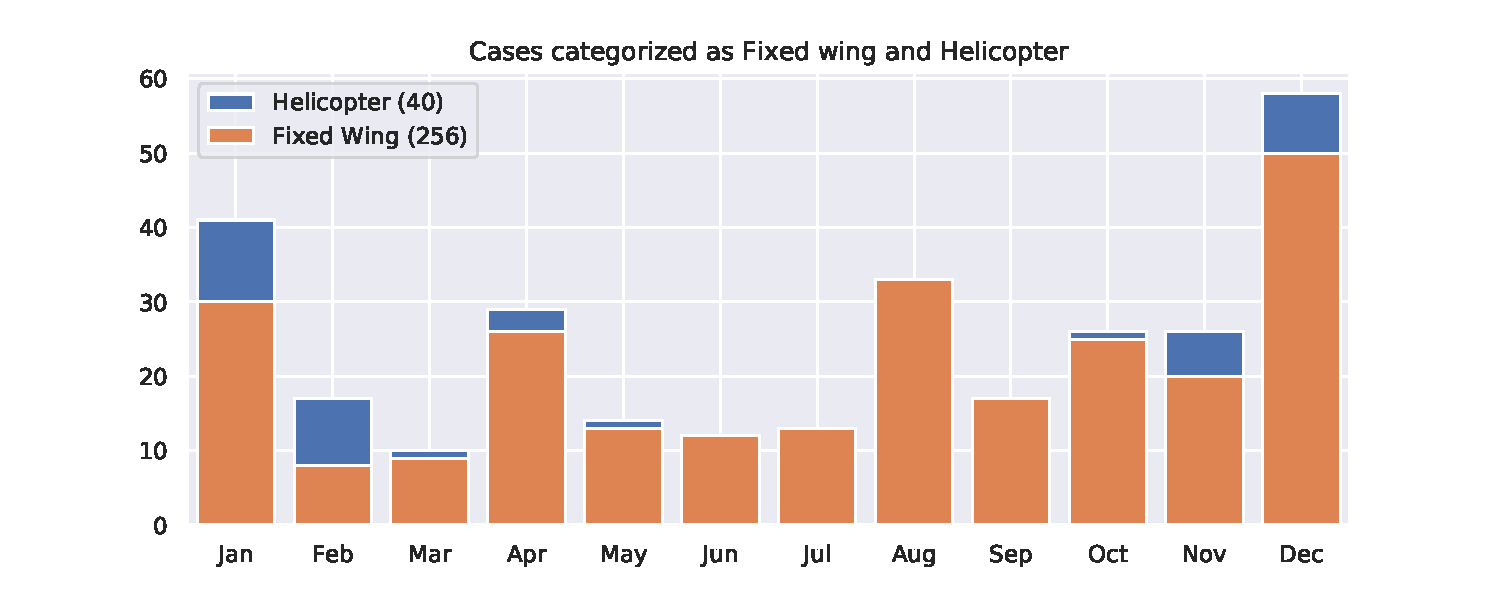
\includegraphics[width=\textwidth]{Figures/helivsfw.pdf}
    \caption{Helicopter and Fixed-wing cases throughout the year}
    \label{fig:helivsfw}
\end{figure}

\begin{figure}
    \centering
    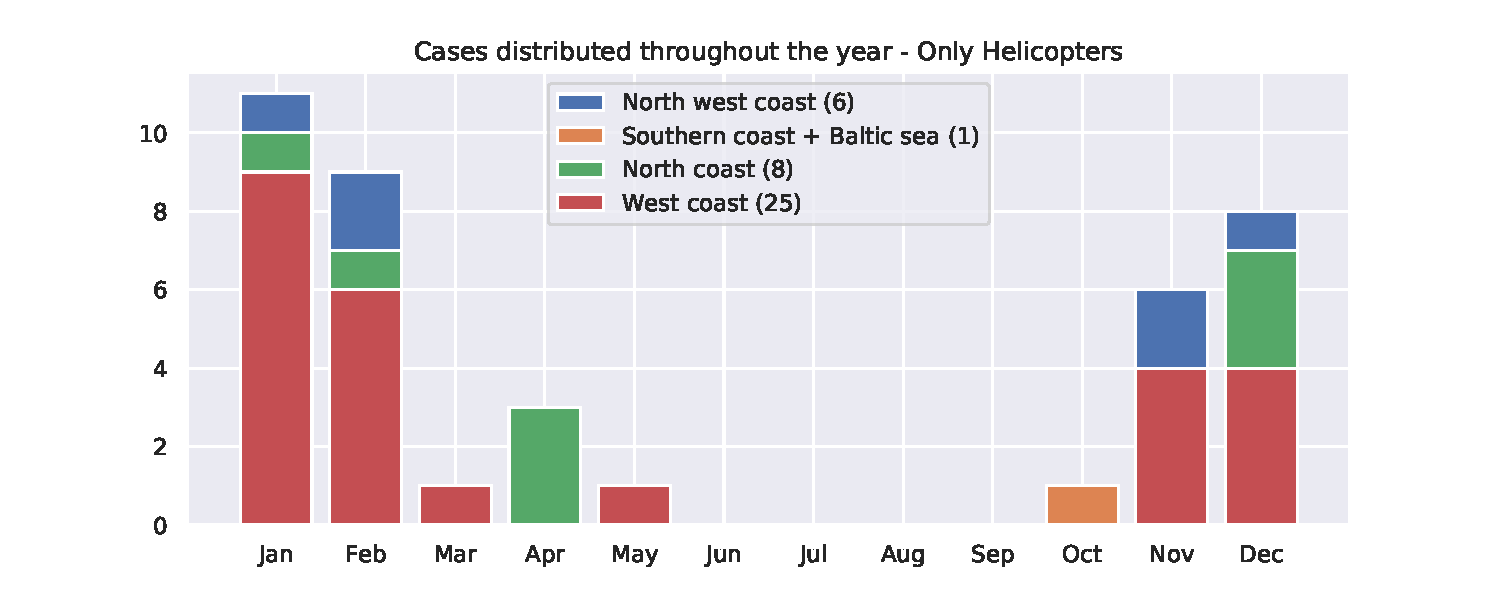
\includegraphics[width=\textwidth]{Figures/Helisoner.pdf}
    \caption{Geographical variation of helicopter cases}
    \label{fig:helisoner}
\end{figure}

\begin{figure}
    \centering
    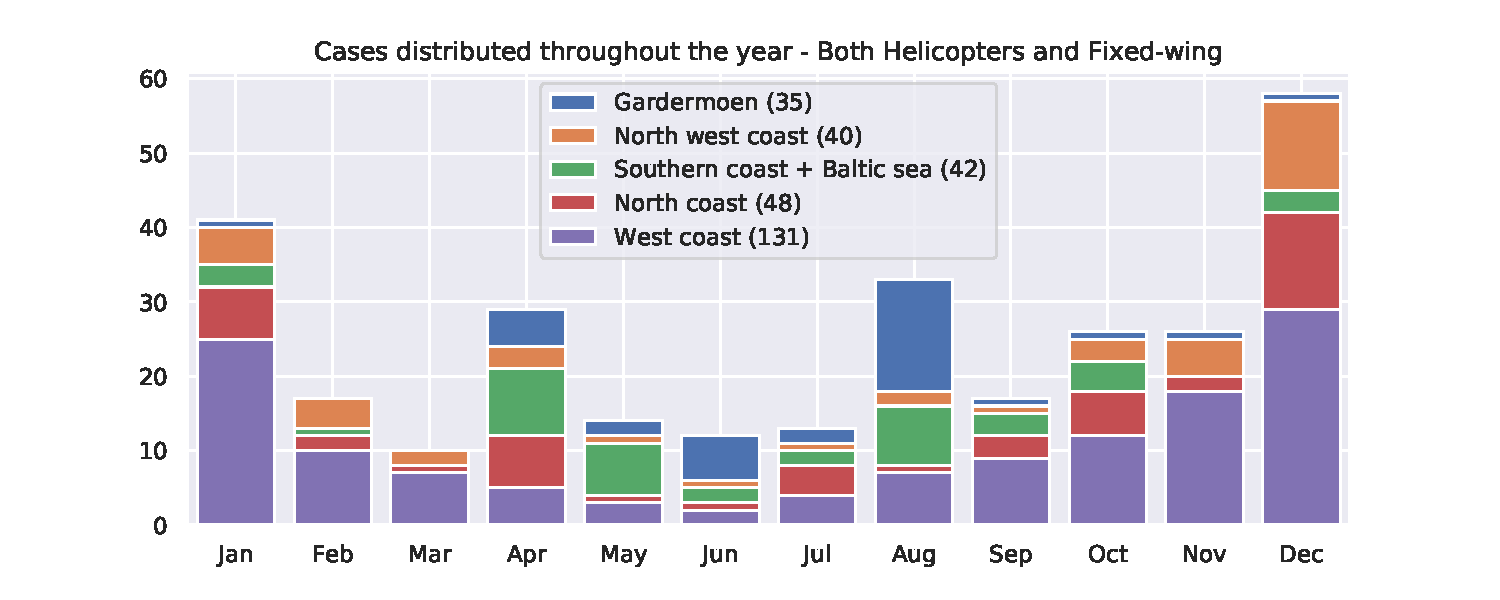
\includegraphics[width=\textwidth]{Figures/soner.pdf}
    \caption{Geographical variation of all cases}
    \label{fig:soner}
\end{figure}

\subsection{METAR}
Figure \ref{fig:metarclimat} shows the frequency of observed meteorological phenomena at a selection of Norwegian airports for the \acrshort{htl}-season. We see generally few reports of hail (GS) and some variation in the amount of cumulonimbus clouds (CB). For Gardermoen, which is not a coastal airport, we see almost no cumulonimbus clouds reported during the winter season. This is also true for the shower (SH) and shower vicinity (VCSH) phenomena. This is to be expected, as Gardermoen is inland and therefore subject to wintertime inversions. This inversion is not present along the coast of Norway due to the North Atlantic Current. We also see that there are few cases where overcast (OVC) is reported along the coast, which further supports the previous statement about inversions. As we move north along the coast, from Sola to Hammerfest, we see that the frequency of snow (SN) increases. This indicates a colder atmosphere.


\begin{figure}
    \centering
    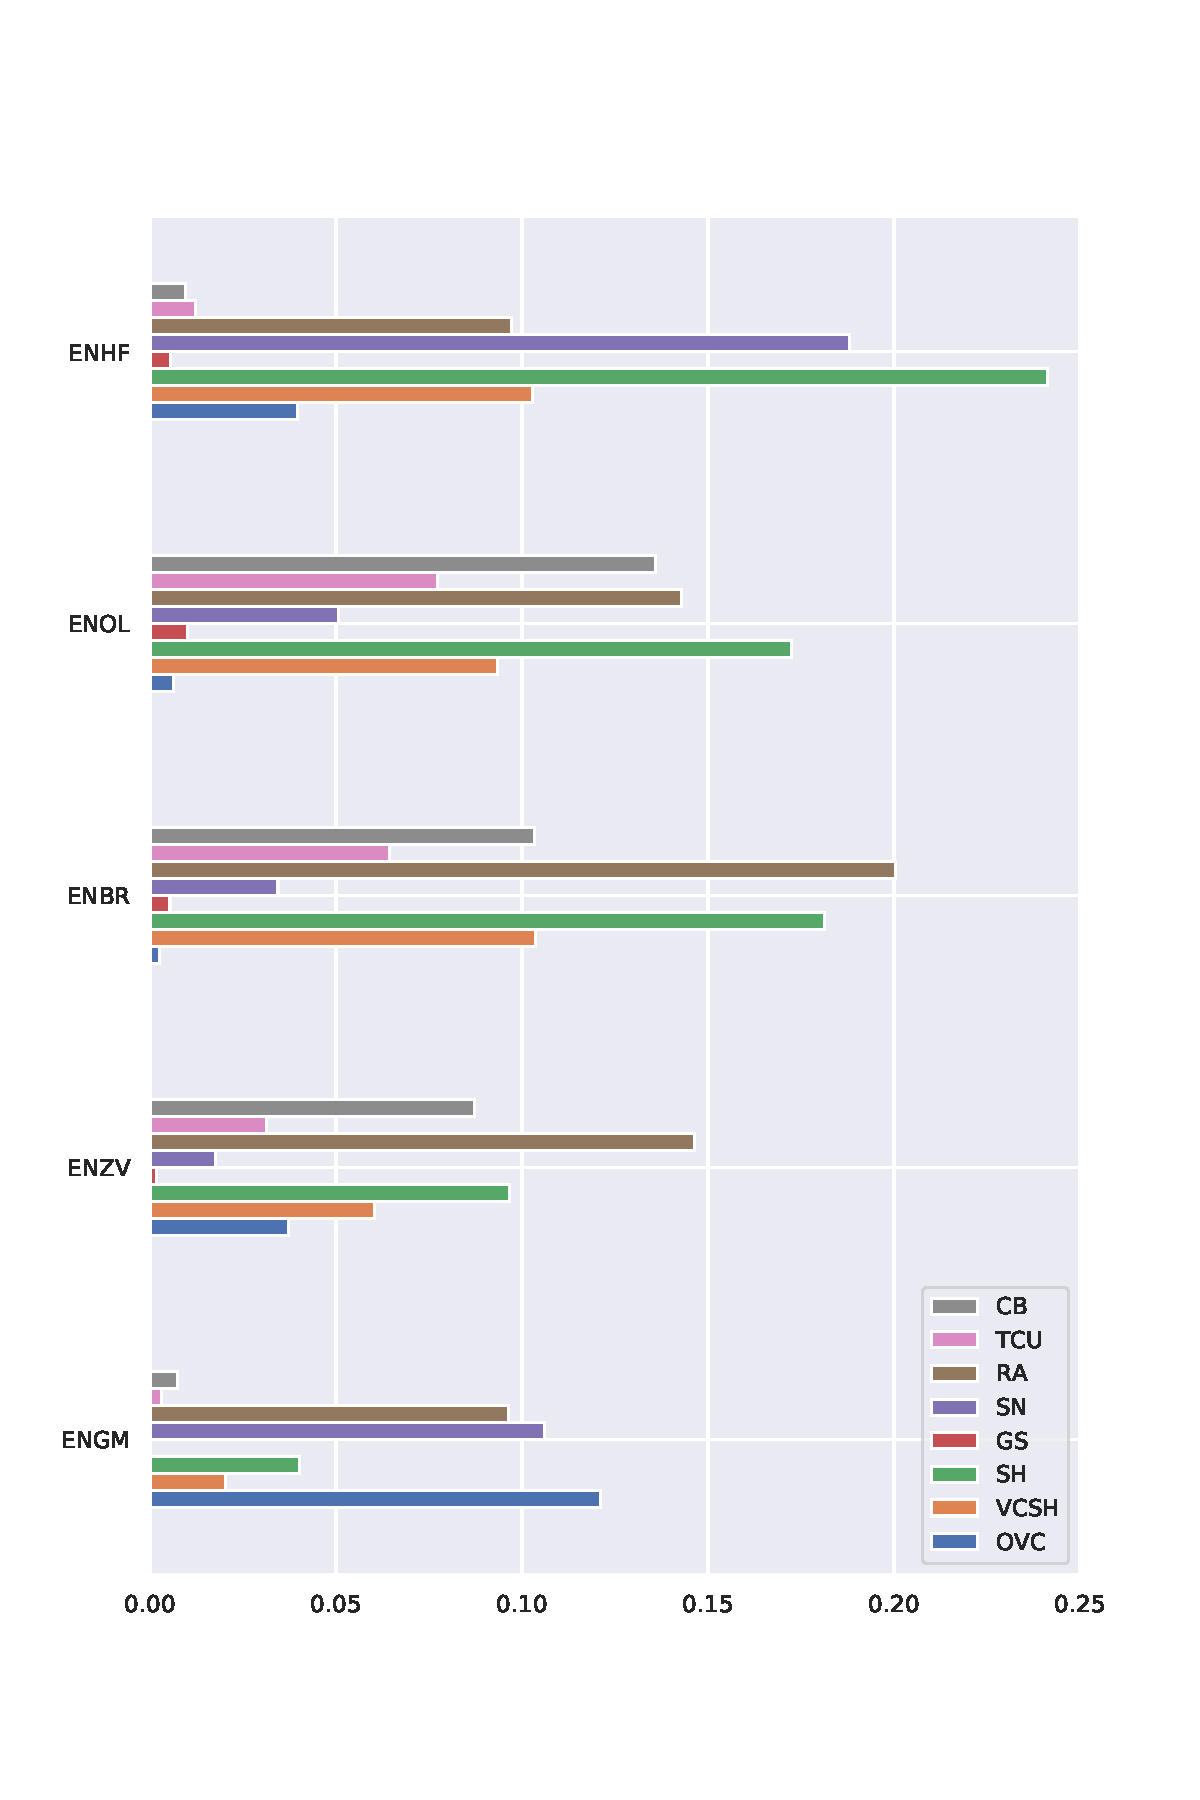
\includegraphics[width=\textwidth]{Figures/METAR_airports.pdf}
    \caption{METAR climatology}
    \label{fig:metarclimat}
\end{figure}

Figure \ref{fig:metarcases} shows the frequency of observed meteorological phenomena when helicopter and fixed-wing cases are reported. Here we see a smaller frequency of relevant meteorological phenomena (cumulonimbus, showers and shower vicinity) for helicopter cases compared to fixed-wing cases. We also see that the frequency of snow and rain is somewhat equal for the helicopter cases, while for the fixed-wing cases there are more cases where rain is reported and not snow. This may be a result of fixed-wing cases being an all-year phenomenon, so that snow is hardly reported.

\begin{figure}
    \centering
    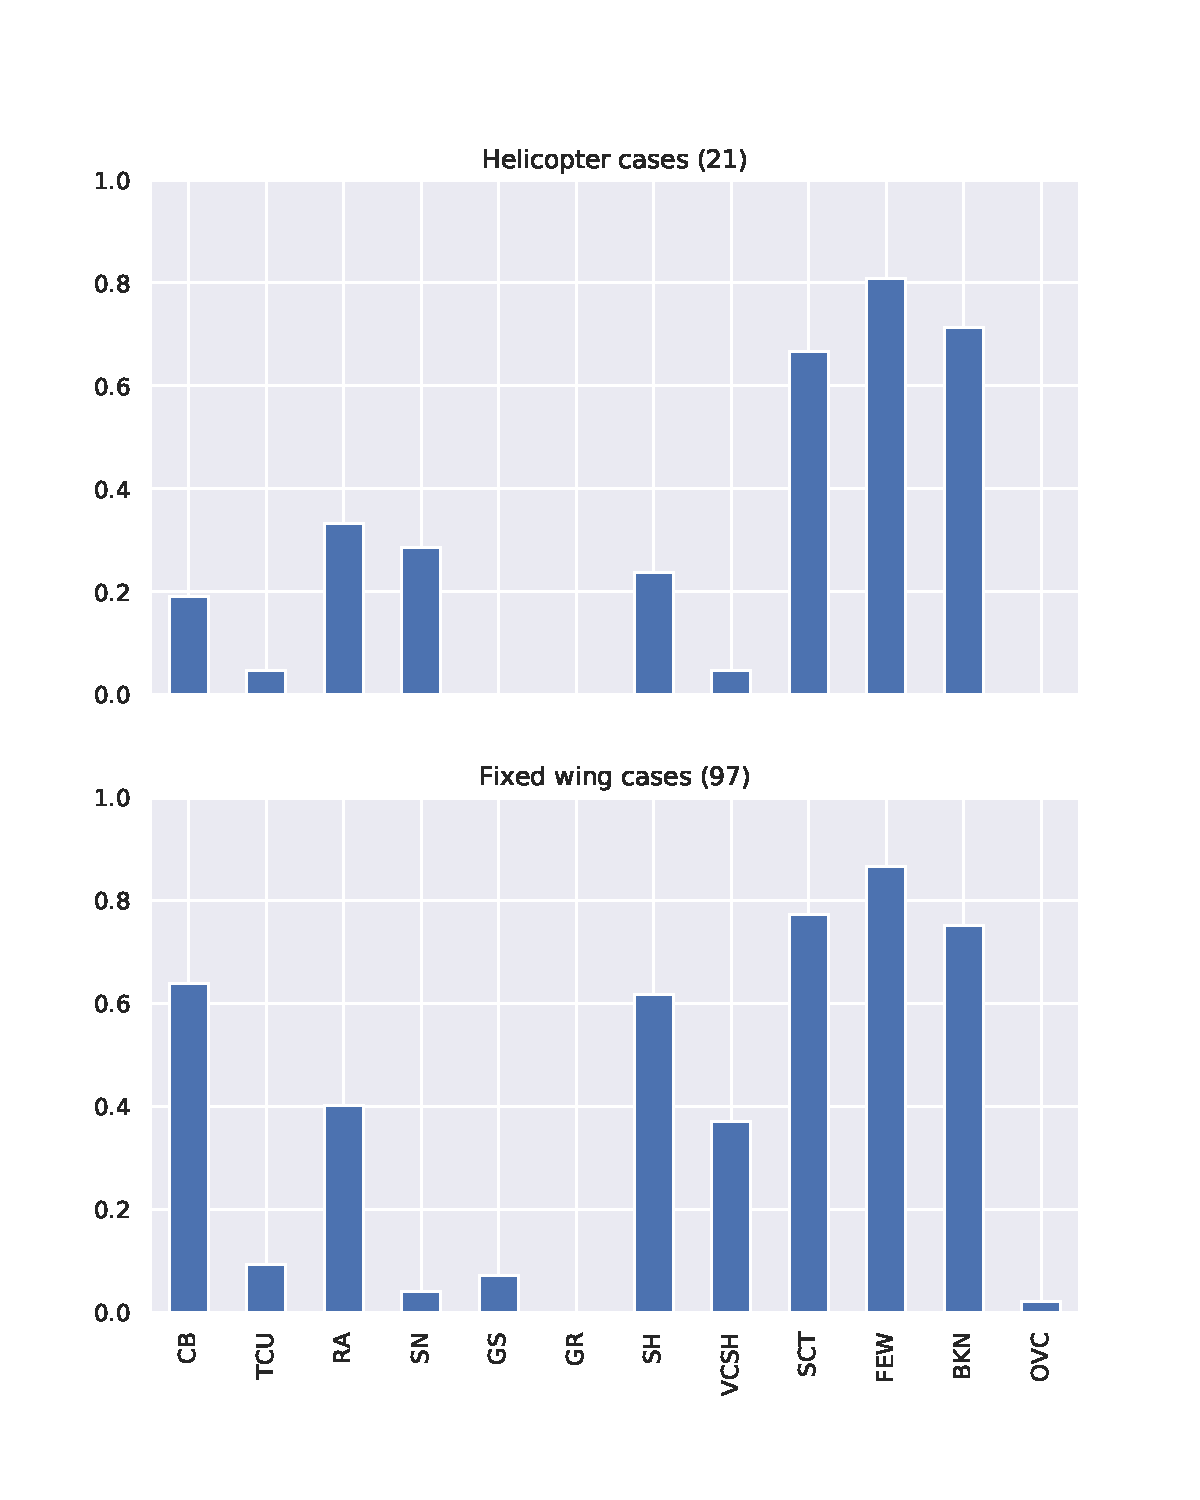
\includegraphics[width=\textwidth]{Figures/METARcases.pdf}
    \caption{METAR for cases}
    \label{fig:metarcases}
\end{figure}

\begin{table}
        \begin{tabular}{r|l|l|l|}
            & Sola (ENZV) & Flesland (ENBR) & Gardermoen (ENGM) \\\hline
            Average Traffic (2016-2018)  & 74 532 & 92 128 & 253 599   \\\hline
            Lightning close to airport (2008-2018) & 78 008 & 70 813   & 186 074 \\\hline
            Cases close to airport & 24 & 63  & 35 \\\hline
            Case per traffic & 1 / 31 050 & 1 / 14 620 & 1 / 72 460\\\hline
            Lightning per case & 32 500 & 11 240 & 53 160 \\\hline
        \end{tabular}
     \caption{Average traffic related to lightning and lightning related cases, for the three biggest airports by traffic-data for 2016-2018}
     \label{tab:traffic}
\end{table}

\section{ERA5 climatologies and cases data}\label{sec:era5results}
For each case in the Avinor dataset the temperature is estimated by interpolation (as discussed in \ref{sec:interpolation}) from \acrshort{era5} pressure level temperature data as shown in Figure \ref{fig:temperatureera5}. The cases include both \acrshort{fwtl} and \acrshort{htl}. The temperature distribution is normal-like around -1C. These cases may include both induced and triggered lightning, which may explain the cases happening at above 2C as these may happen under the electrically active area. It is worth noting that most of the cases happen in the -10C to 0C temperature range, where the electrification process is believed to be most active. There is also a similarity between the distributions for \acrshort{htl} and \acrshort{fwtl} cases. This hints that the phenomena are closely related, as discussed later.

Further, Figure \ref{fig:meaneraT750} shows the mean climatological temperature of the \acrshort{htl} season for 2008-2019 for 750 meters above sea level. This shows that the temperature along the coast of Norway is around 0C to -5C during the \acrshort{htl} season, which we saw from Figure \ref{fig:temperatureera5} is where most triggered lightning happens. Linking this to the mean sea surface temperature, as shown in Figure \ref{fig:meanerasst}, we see that the sea surface is around 5C to 10C on the Norwegian coast during \acrshort{htl} season. This results in a climatological lapse rate of $-\frac{5 \text{ to } 10 ^{\circ}C}{750m} \approx -\frac{6.67 \text{ to }13.33 ^{\circ}C}{km}$. Compared to the dry adiabatic lapse rate, of -9.8C/km, this would be on the lower end of the climatological lapse rate approximation lead to a stable atmosphere, while on the higher end to an unstable atmosphere - if the air was dry. However, since this is above the open sea, relative humidity will lower the required magnitude of the temperature gradient for an unstable atmosphere. 

\begin{figure}
    \centering
    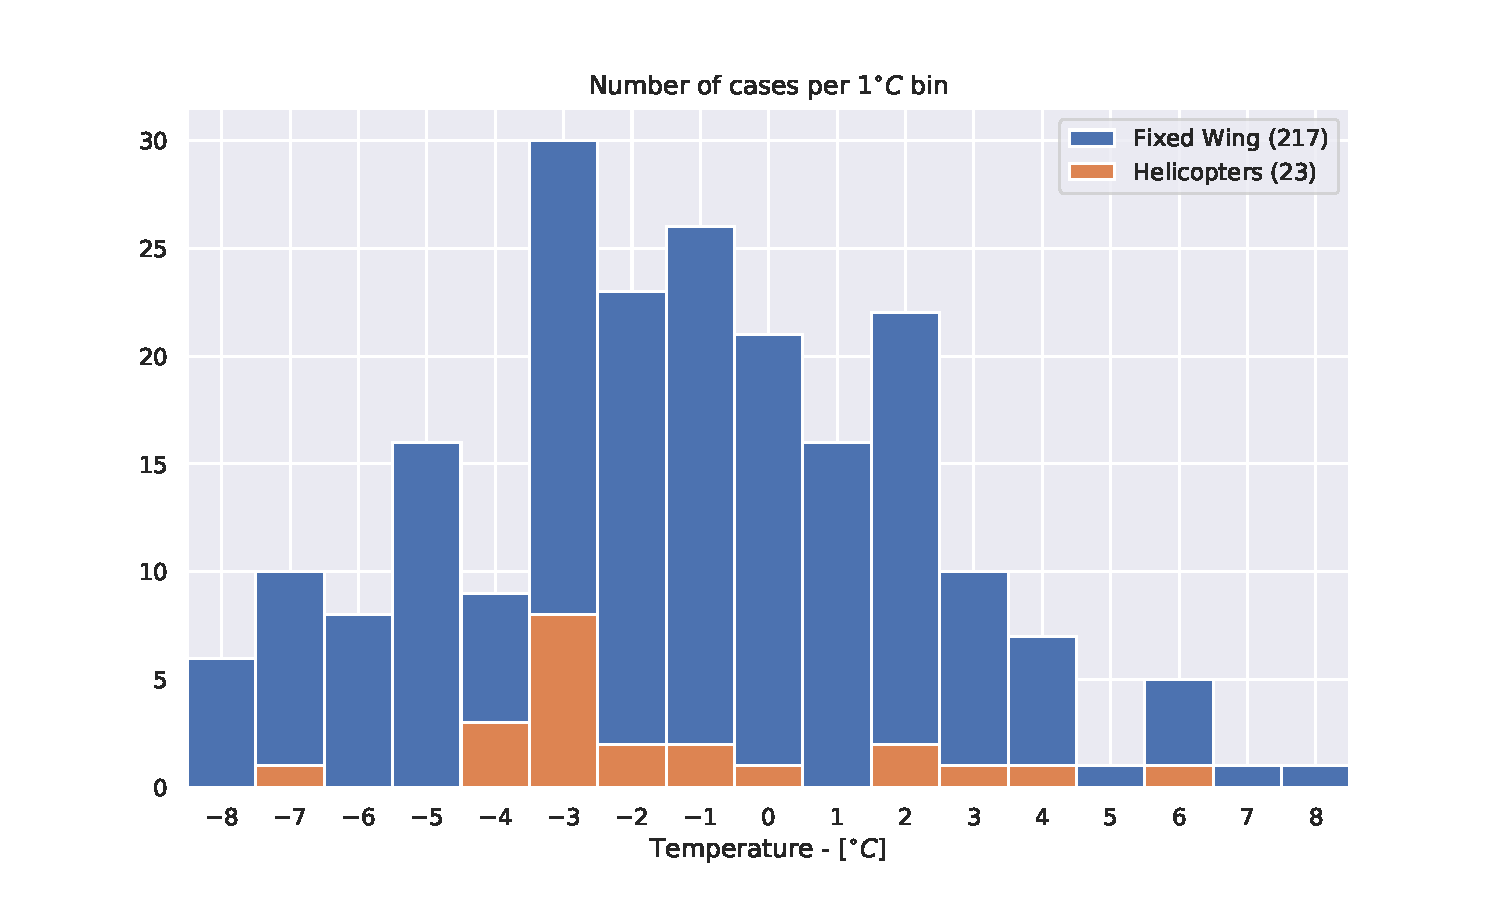
\includegraphics[width=\textwidth]{Figures/temperature.pdf}
    \caption{Temperature in fixed-wing and helicopter cases (interpolated from ERA5 pressure levels)}
    \label{fig:temperatureera5}
\end{figure}

\begin{figure}
    \centering
    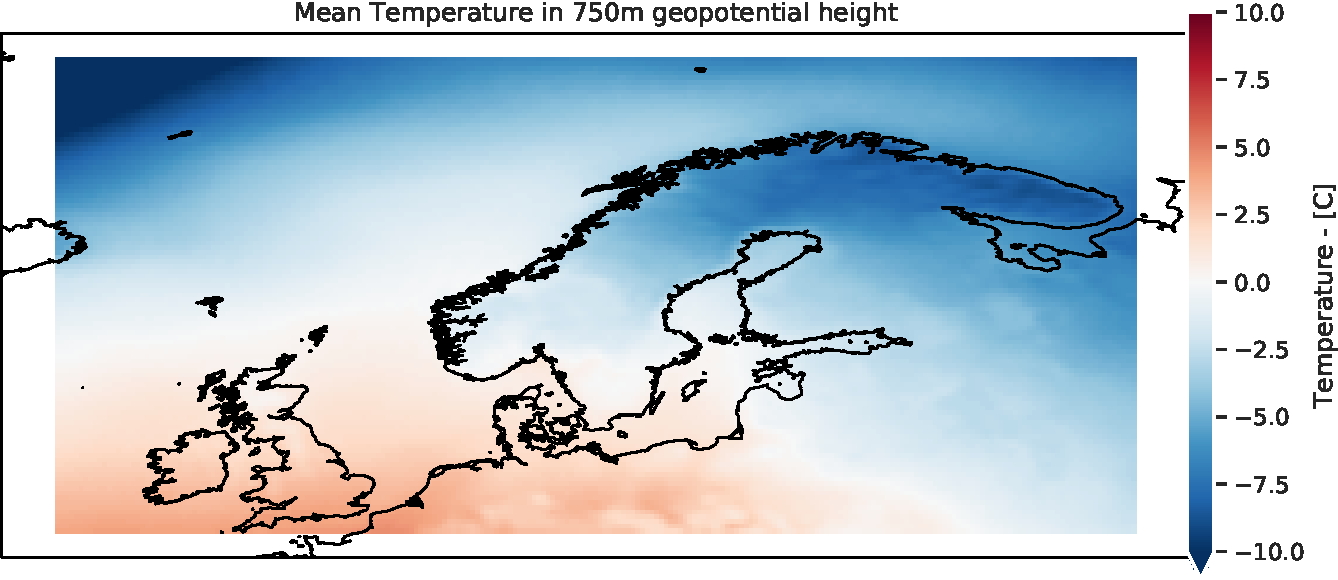
\includegraphics[width=\textwidth]{Figures/MeanT750era5.pdf}
    \caption{Mean Temperature of 750m height in HTL season (ERA5)}
    \label{fig:meaneraT750}
\end{figure}

\begin{figure}
    \centering
    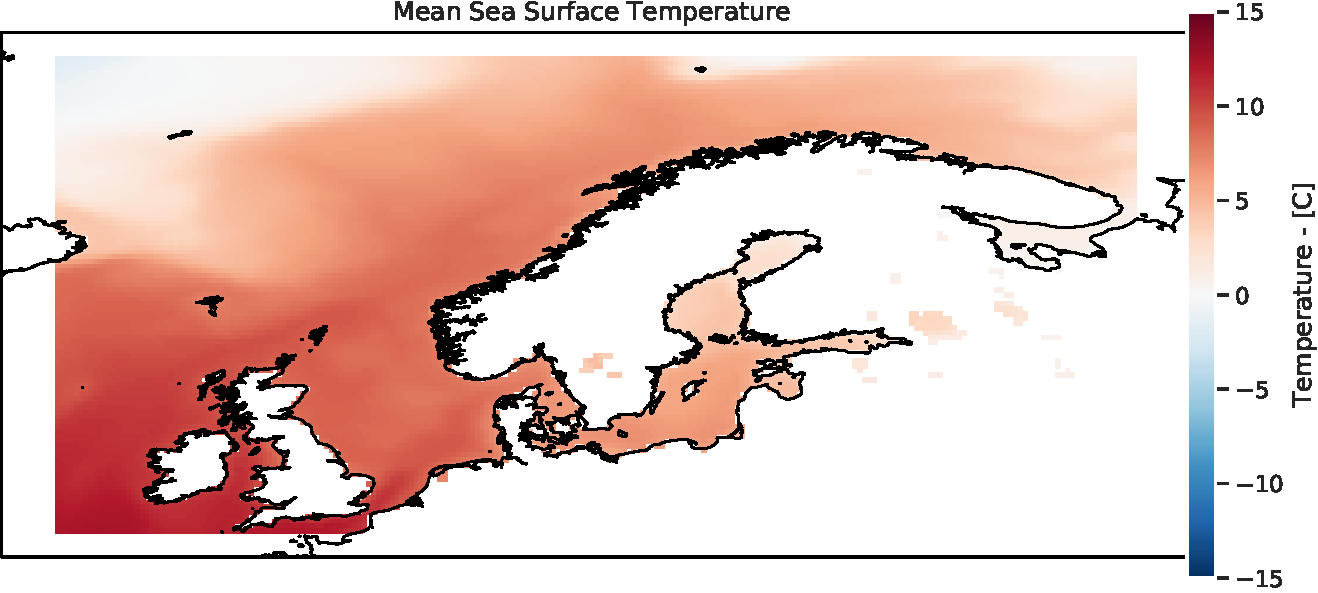
\includegraphics[width=\textwidth]{Figures/MeanSSTera5.pdf}
    \caption{Mean Sea Surface Temperature (SST) in HTL season (ERA5)}
    \label{fig:meanerasst}
\end{figure}

\subsection{Composites of parameters used in forecasting divided by zone}
In this section we investigate the different components contributing to the index used in forecasting risk for \acrlong{htl}. Note that the cloud-cover variable has been moved to the A-appendix, due to it showing no clear signal, due to the horizontal sparseness of ERA5 compared to MEPS.

\subsubsection{Temperature}
Figure \ref{fig:tempzones} shows the mean temperature for the cases in each zone above the standard deviation for the temperature in each zone. These are made by using the height information and the time information of the cases in each zone. 

We see from Figure \ref{fig:NordTemperature} that the mean temperature in 750 meters height (the level used in \acrshort{htl} forecast) is below zero for the cases in the North, stretching from the cases in Hammerfest in the northeast to the cases in Brønnøysund, in the southern part of the northernmost zone. We also see that there is some variation in the temperature of the northern zone. This is most likely caused by the geographical spread of these cases. It is far from Hammerfest to Brønnøysund. The pressure shows a low in the Barents Sea, making the general wind patterns for these cases to be incident on the shore of the coast of Northern Norway. This makes cold dry air with an Arctic origin develop into convection which finally is reinforced by converging along the Norwegian coast. 

Moving to the northwest zone in Figure \ref{fig:NordWestTemperature}, we see that the low pressure is further to the south and more pronounced (isobars at 992 and 996 hPa compared to 1000 and 1004 hPa in the north.) The latter is probably due to less spatial variation in the northwest zone than in the north zone. This is also seen in the standard deviance plots for both temperature and pressure. The temperature here is also on the colder side of zero, but the isotherms are moved southward so that the cases are happening around -1C to 0C. Again we see on-shore air flow which may have originated in the Arctic due to geostrophic wind patterns (along the isobars).

The now-familiar trend is repeated for the west case, seen in Figure \ref{fig:WestTemperature}. A low pressure which gives winds incident on the west coast of Norway is situated over the sea. We also see that the temperature range, the isotherms have moved further south so that the temperature range -3C to 0C is now situated on the west coast of Norway. Here we also see some variance in the temperature, but least variance around the west coast. 

In Figure \ref{fig:SouthTemperature} we see that the isotherms follow the zone such that the -3C to 0C degree range seem to be situated around the airports where we have incidents. Though we also see that the variance is also largest here, due to the big geographical spread present as well. Here we do not see a very clear signal in the pressure. A hint at a low pressure over the North Sea, although not very deep. This can also be explained by the big variance of pressure over the ocean for these cases 

In total, Figure \ref{fig:tempzones} shows that the cases are within the same temperature ranges as expected from earlier studies, although some variation in the larger zones, here north and south. There is also a clear trend in the pressure systems to be causing geostrophic winds incident on the coasts.

\begin{figure}
\begin{subfigure}[b]{0.49\textwidth}
    \centering
    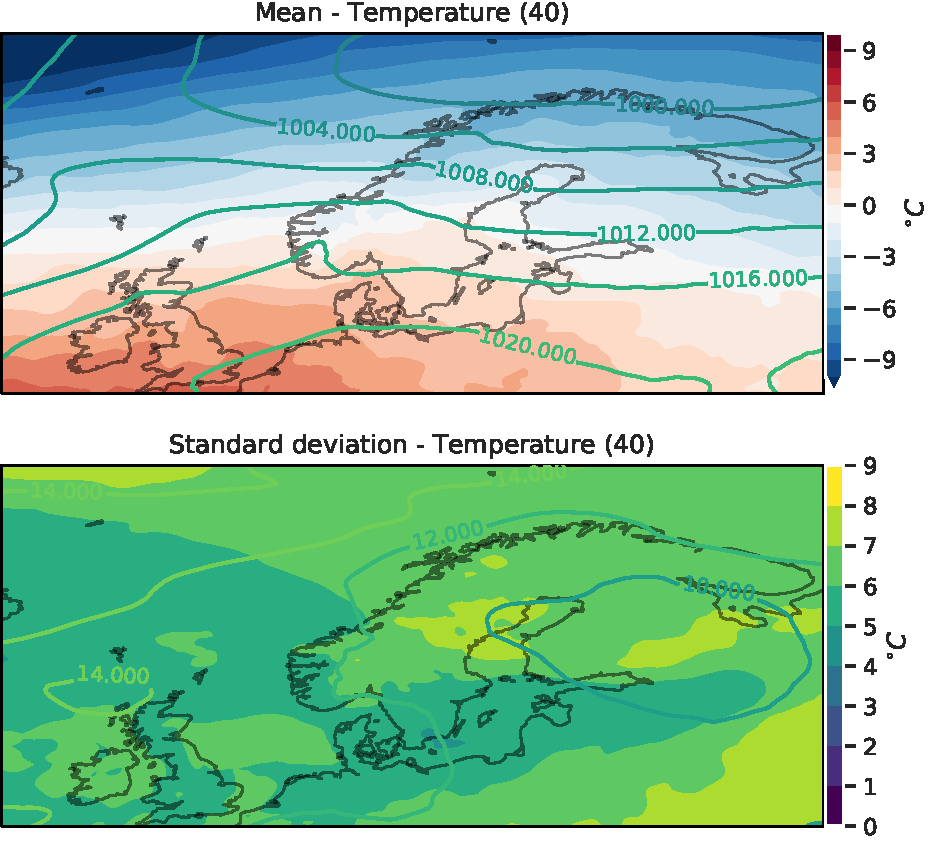
\includegraphics[width=\textwidth]{Figures/TempNord.pdf}
    \caption{Temperature for cases in North zone.}
    \label{fig:NordTemperature}
\end{subfigure}
\begin{subfigure}[b]{0.49\textwidth}
    \centering
    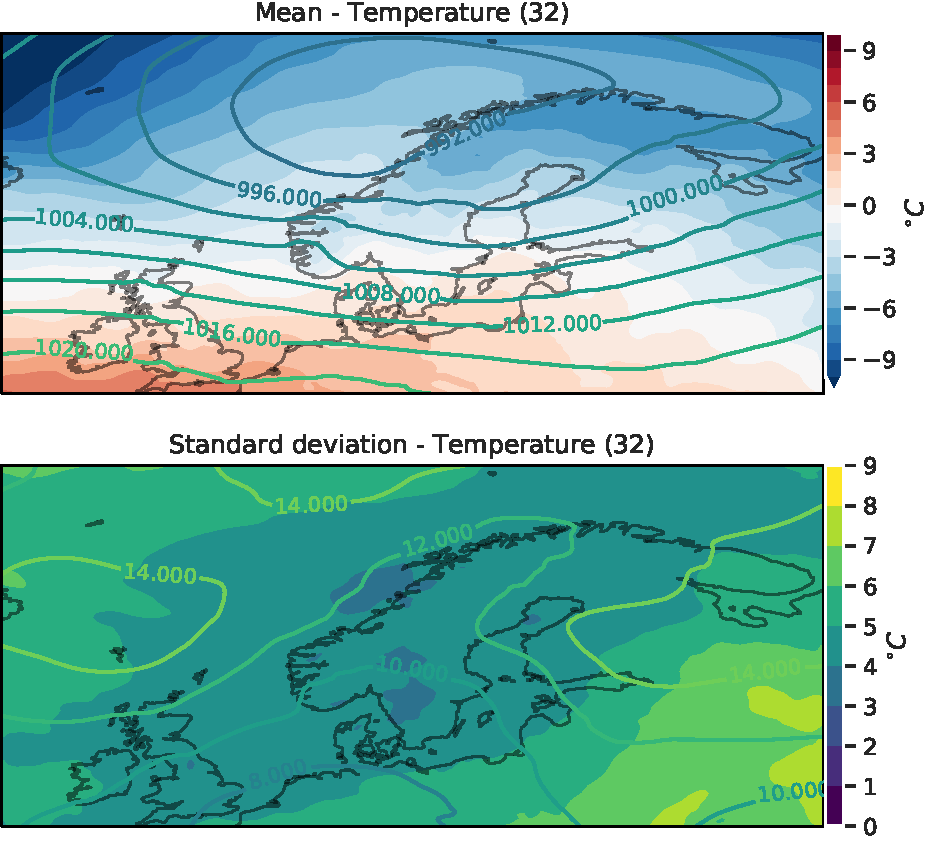
\includegraphics[width=\textwidth]{Figures/TempNordvest.pdf}
    \caption{Temperature for cases in Northwest zone.}
    \label{fig:NordWestTemperature}
\end{subfigure}
\begin{subfigure}[b]{0.49\textwidth}
    \centering
    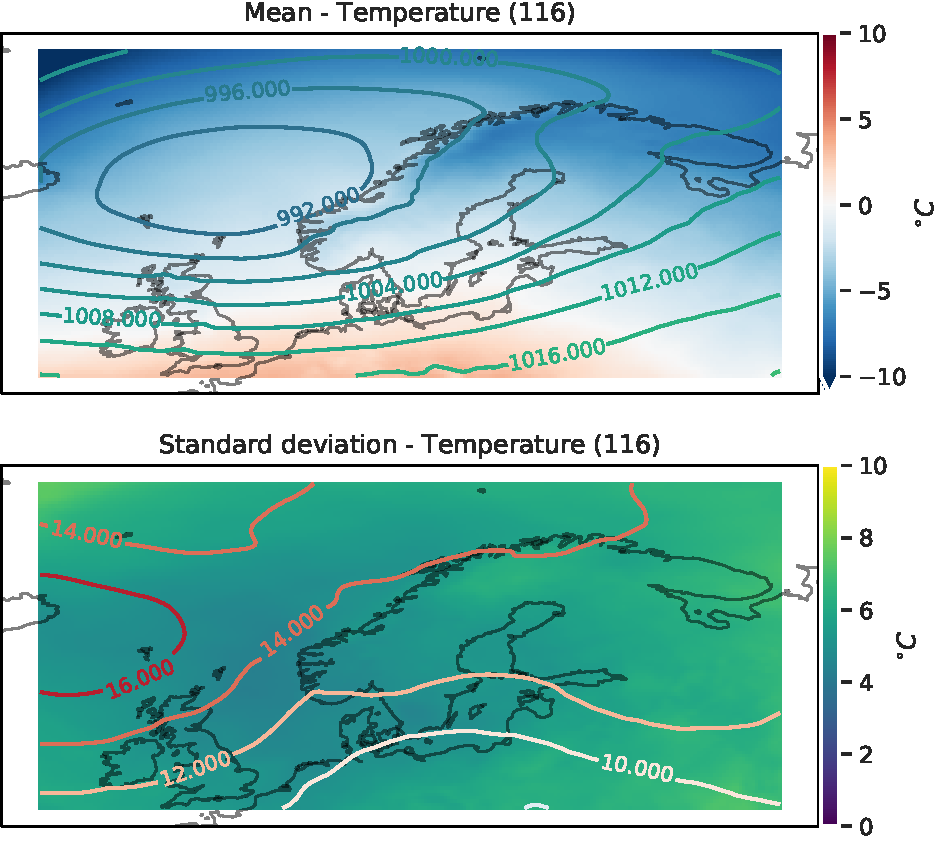
\includegraphics[width=\textwidth]{Figures/TempVest.pdf}
    \caption{Temperature for cases in West zone.}
    \label{fig:WestTemperature}
\end{subfigure}
\begin{subfigure}[b]{0.49\textwidth}
    \centering
    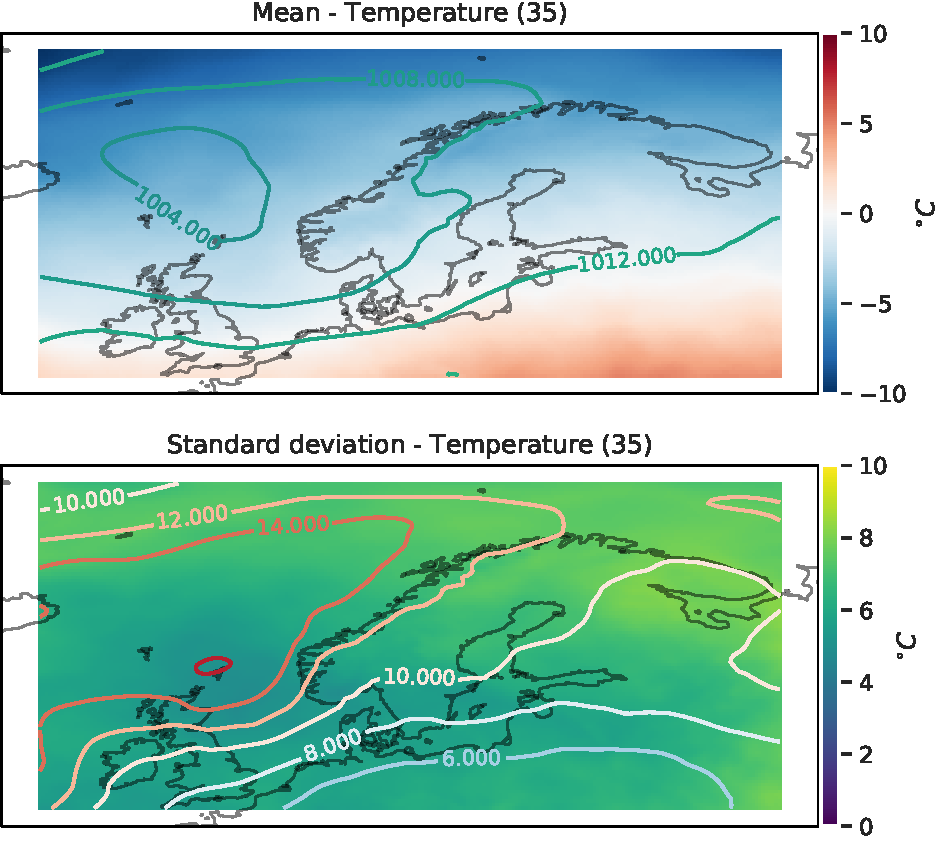
\includegraphics[width=\textwidth]{Figures/TempSor.pdf}
    \caption{Temperature for cases in South zone.}
    \label{fig:SouthTemperature}
\end{subfigure}
\caption{Temperature composites for the different zones}
\label{fig:tempzones}
\end{figure}

Looking, then, on Figure \ref{fig:tempairports}, we see that the cases happening at Flesland airport in \ref{fig:ENBRTemperature} have a very low variation in temperature, but some variation in the pressure systems. The average situation shows a deep pressure system over the North Sea (988 hPa) and temperatures around -1C. 

The same pattern is present for the Sola airport in Figure \ref{fig:ENZVTemperature}: Temperatures are around 0C, but also here there is some variation in the pressure system. Though this may be due to placement of the low pressure systems and not the actual magnitude. 

Looking at Gardermoen in Figure \ref{fig:ENGMTemperature} we see a much warmer average situation around 2C, and with more variation in the temperature. And the pressure system does not seem to be either very high nor low being around 1006 hPa. Also, there seems to be very little variation in the pressure for Gardermoen. It should be noted that Figure \ref{fig:yearlyvariation} shows that Gardermoen is relatively unique compared to the other zones, in that cases occur mainly during the summer season.

\begin{figure}
     \centering
     \begin{subfigure}[b]{0.49\textwidth}
         \centering
         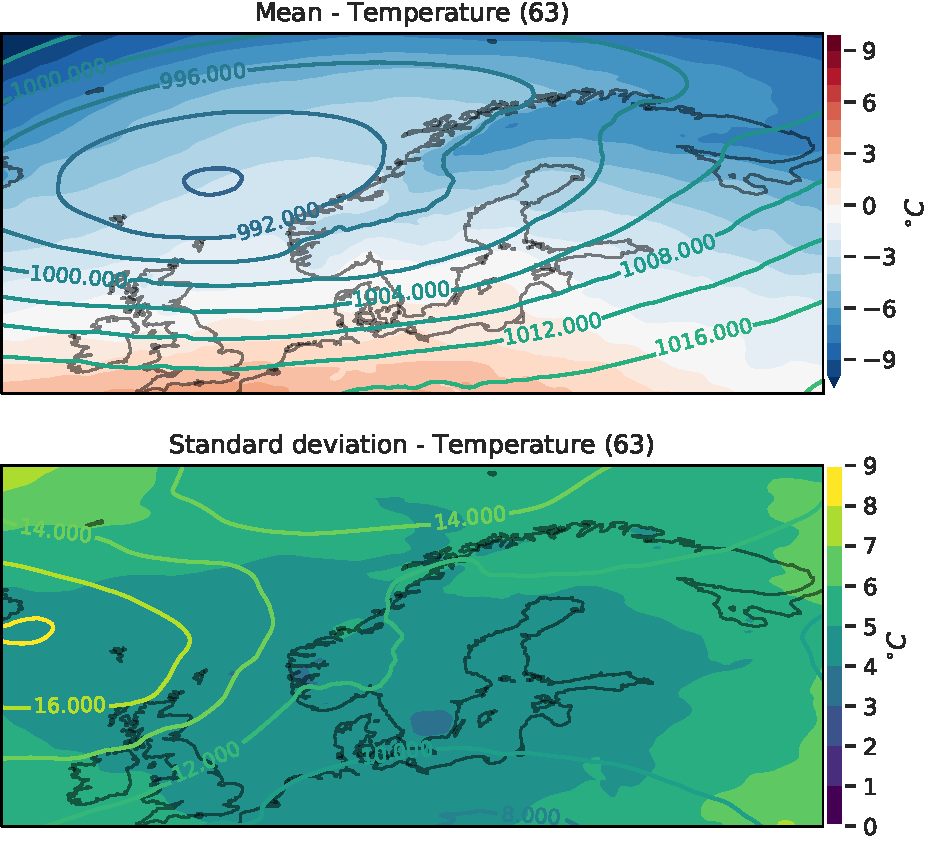
\includegraphics[width=\textwidth]{Figures/TempENBR.pdf}
         \caption{}
         \label{fig:ENBRTemperature}
     \end{subfigure}
     \hfill
     \begin{subfigure}[b]{0.49\textwidth}
         \centering
         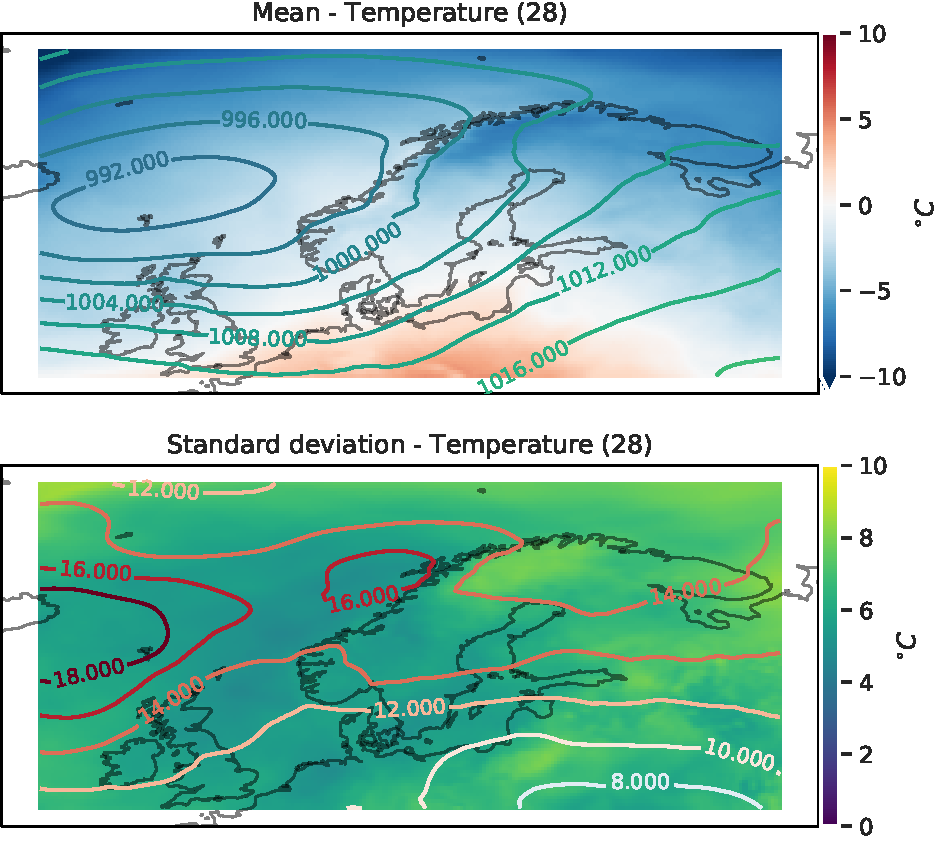
\includegraphics[width=\textwidth]{Figures/TempENZV.pdf}
         \caption{}
         \label{fig:ENZVTemperature}
     \end{subfigure}
     
    \begin{subfigure}[b]{0.5\textwidth}
    \centering
    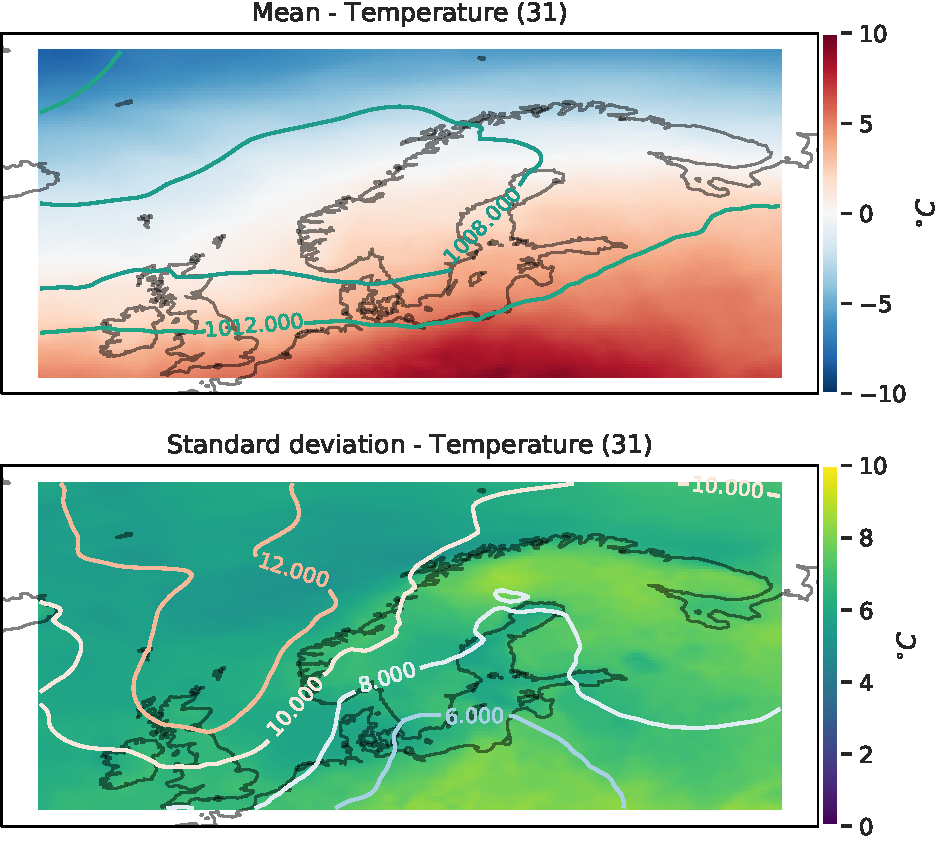
\includegraphics[width=\textwidth]{Figures/TempENGM.pdf}
    \caption{Temperature for cases in Gardermoen zone.}
    \label{fig:ENGMTemperature}
\end{subfigure}
\caption{Temperature composites for the biggest airports}
\label{fig:tempairports}
\end{figure}

\subsubsection{Vertical velocity}

Figure \ref{fig:verticalzones} shows the average situation and the standard deviation of the vertical velocity for the cases. Note here that the units are hPa per second, not meters per second, such that a positive value refers to a downwelling of airmass and a negative value an upwelling. It is important to recall the discussion in \ref{sec:models} that \acrshort{era5} is coarser in its horizontal resolution such that it should not necessarily produce very strong vertical velocities, i.e. local convection may be lost in \acrshort{era5}.

In Figure \ref{fig:NordW} we see that there is a signal of upward velocity along the coast of Nordland fylke and a hint at a signal along the western part of Finnmark and Troms. We also see that there is some variance which is highest around Nordland, suggesting that the placement of these vertical velocity events are varying. This is to be expected because the position of our cases are varying considerably within the region.

Moving to the \ref{fig:NordWestW} we see a clear pattern of upward velocity situated along the northwestern coast. Here also we see the variance is somewhat high around the northwestern coast. This, too, may be caused by the variation of the cases, especially since vertical velocity is a more local and less continuous field than temperature. 

Moving to the west, in Figure \ref{fig:WestW} we see a clear signal of upward velocity along the west coast for these cases. Although the variance is high for these cases, this is most likely a result of the placement of these vertical velocities. An upward velocity causing an HTL at Flesland may be accompanied by a downward velocity in another place along the west coast. It is also to note that the variance is higher in numerical value than the signal in the composite, which further supports the previous statement about the placement. 

Lastly, we look at Figure \ref{fig:SouthW}. This Figure shows no clear signal for any of the places where we have lightning strikes. And the variance is somewhat higher around Denmark hinting to the somewhat "overrepresentation" of Denmark in the dataset. 

In total, Figure \ref{fig:verticalzones} shows that cases with lightning strikes are associated with an upward velocity and that this upward velocity seems to be correctly placed in the model along the coast. However, there is not a clear signal over the open ocean. This may be due to the fact that convection is either too small or randomly/incorrectly placed off-shore. The variance, as discussed above, is highest for the more significant zones due to placement for the vertical movement. 

\begin{figure}
\begin{subfigure}[b]{0.49\textwidth}
    \centering
    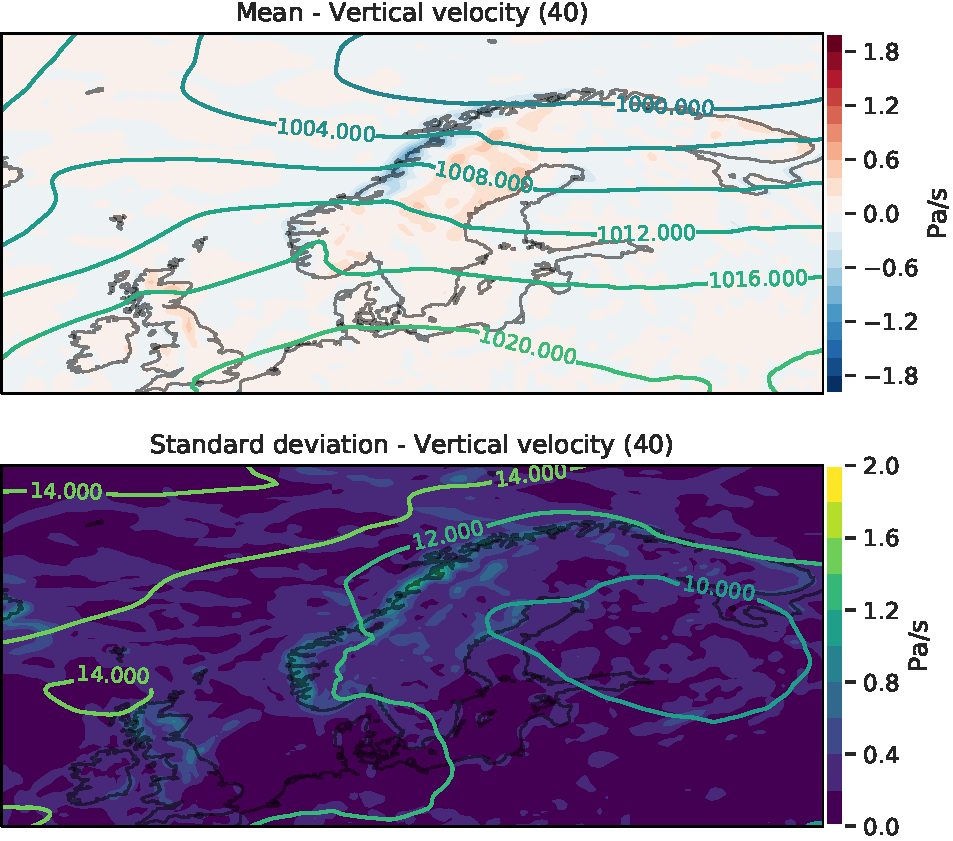
\includegraphics[width=\textwidth]{Figures/WNord.pdf}
    \caption{Temperature for cases in North zone.}
    \label{fig:NordW}
\end{subfigure}
\begin{subfigure}[b]{0.49\textwidth}
    \centering
    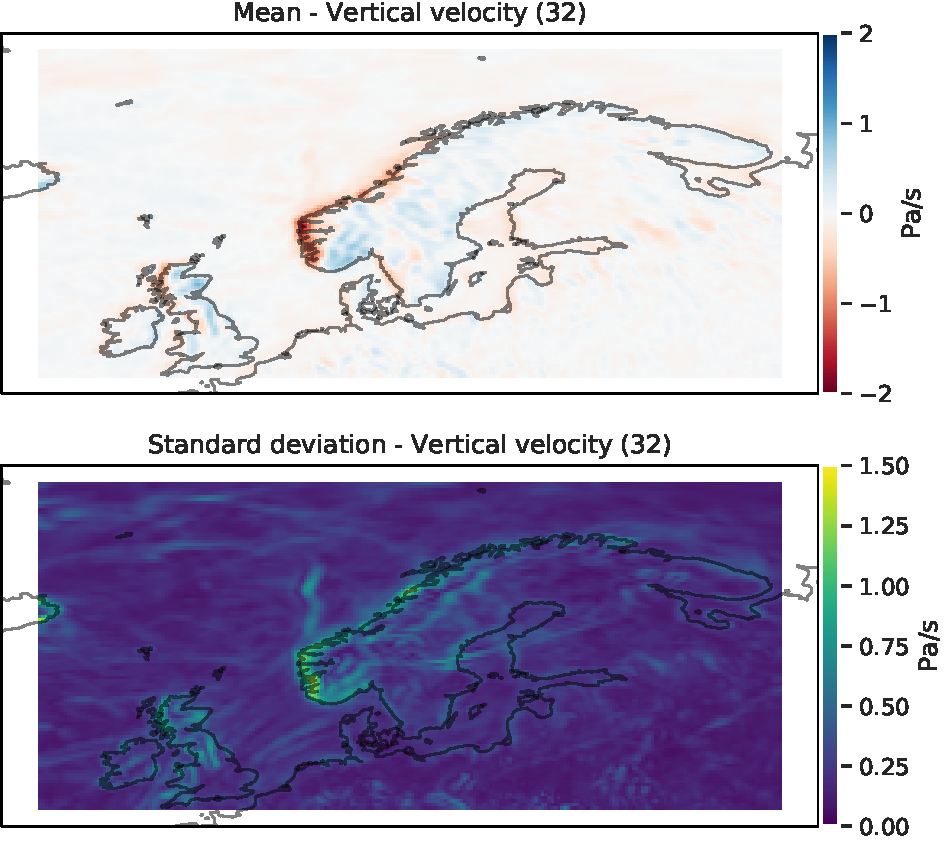
\includegraphics[width=\textwidth]{Figures/WNordvest.pdf}
    \caption{Temperature for cases in Northwest zone.}
    \label{fig:NordWestW}
\end{subfigure}
\begin{subfigure}[b]{0.49\textwidth}
    \centering
    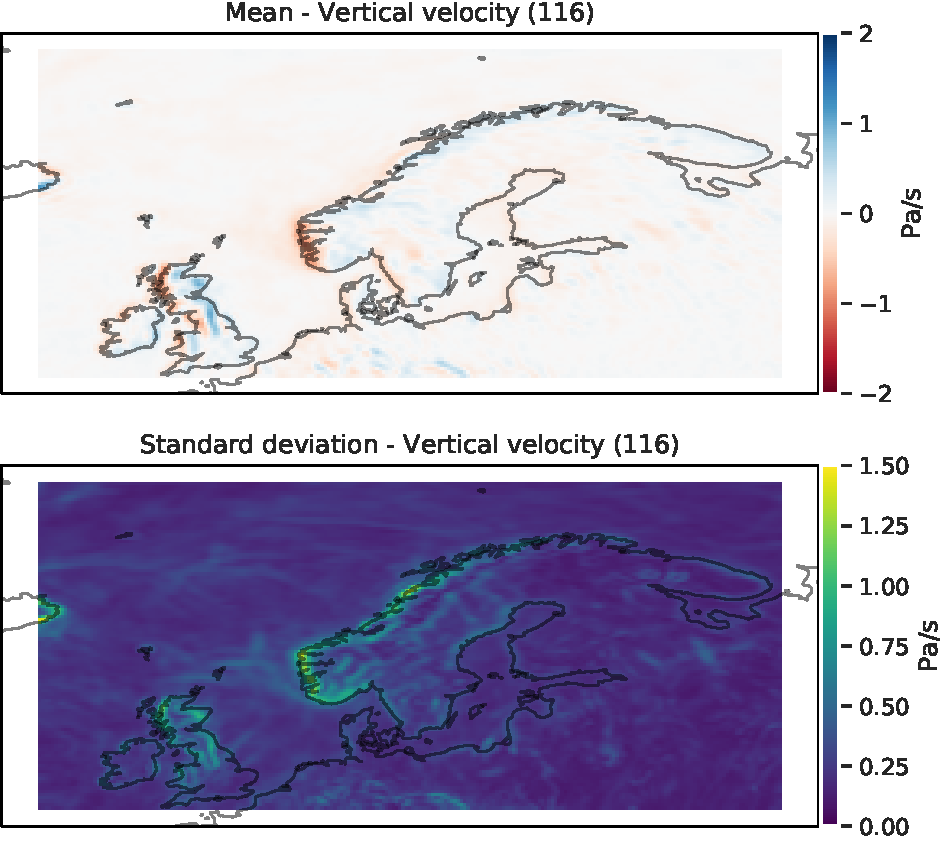
\includegraphics[width=\textwidth]{Figures/WVest.pdf}
    \caption{Temperature for cases in West zone.}
    \label{fig:WestW}
\end{subfigure}
\begin{subfigure}[b]{0.49\textwidth}
    \centering
    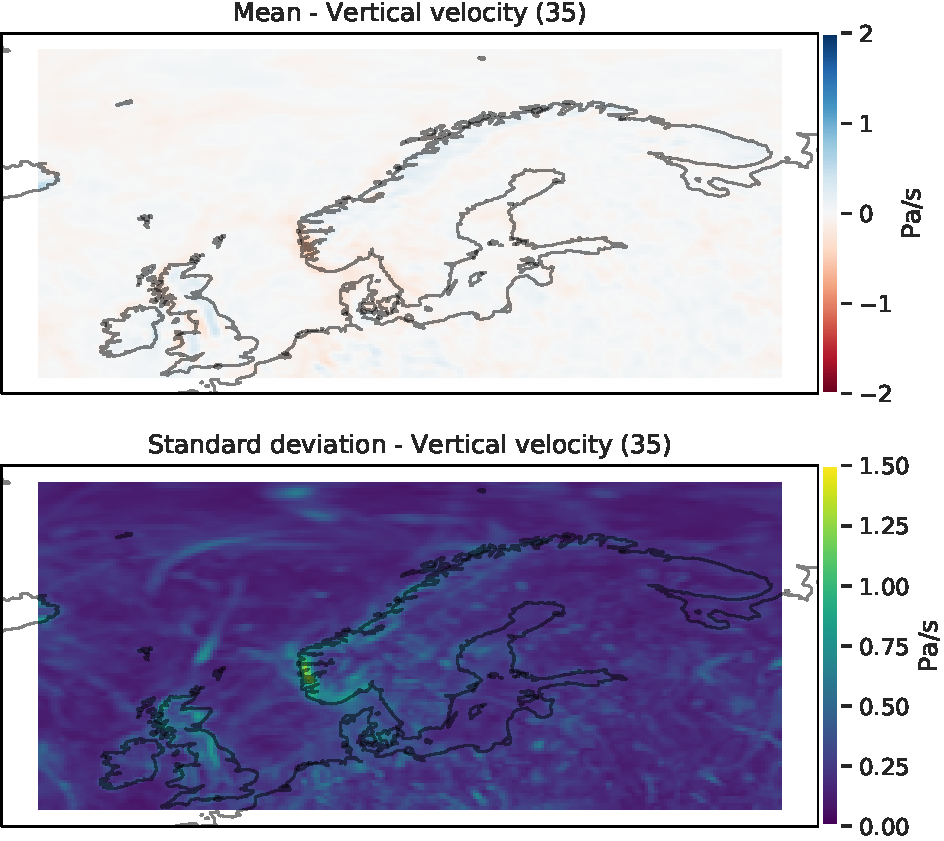
\includegraphics[width=\textwidth]{Figures/WSor.pdf}
    \caption{Temperature for cases in South zone.}
    \label{fig:SouthW}
\end{subfigure}
\caption{Vertical velocity composites for the different zones}
\label{fig:verticalzones}
\end{figure}

This is further confirmed by looking at the biggest airports in Figure \ref{fig:verticalairports}, especially subfigure \ref{fig:ENZVW}, where the standard deviation is highest for the actual placement of Sola airport and the composite shows a clear signal along the west coast. Figure \ref{fig:ENBRW} reinforces this idea, as it shows a clear signal in the composite and some variation along the west coast. Looking at \ref{fig:ENGMW} we see no clear signal for the vertical updraft for Gardermoen airport although we see some variance situated around the airport. This may be because these are summer cases and may be due to \textit{very} local convective system in form of showers.

\begin{figure}
     \centering
     \begin{subfigure}[b]{0.49\textwidth}
         \centering
         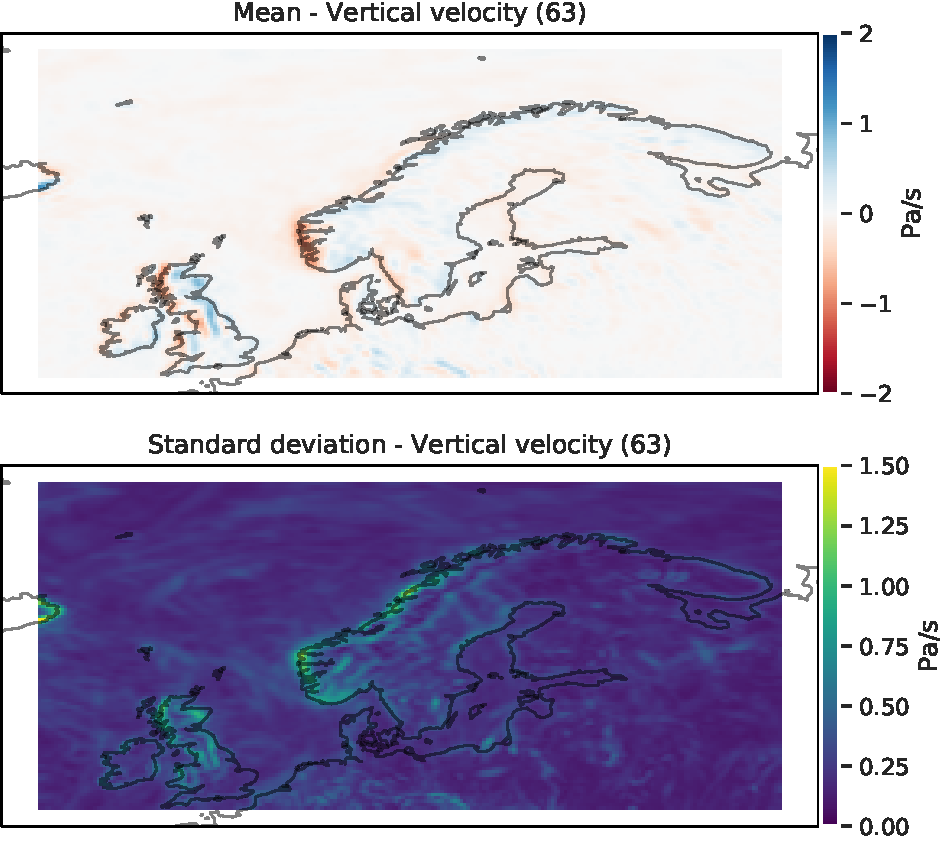
\includegraphics[width=\textwidth]{Figures/WENBR.pdf}
         \caption{Flesland}
         \label{fig:ENBRW}
     \end{subfigure}
     \hfill
     \begin{subfigure}[b]{0.49\textwidth}
         \centering
         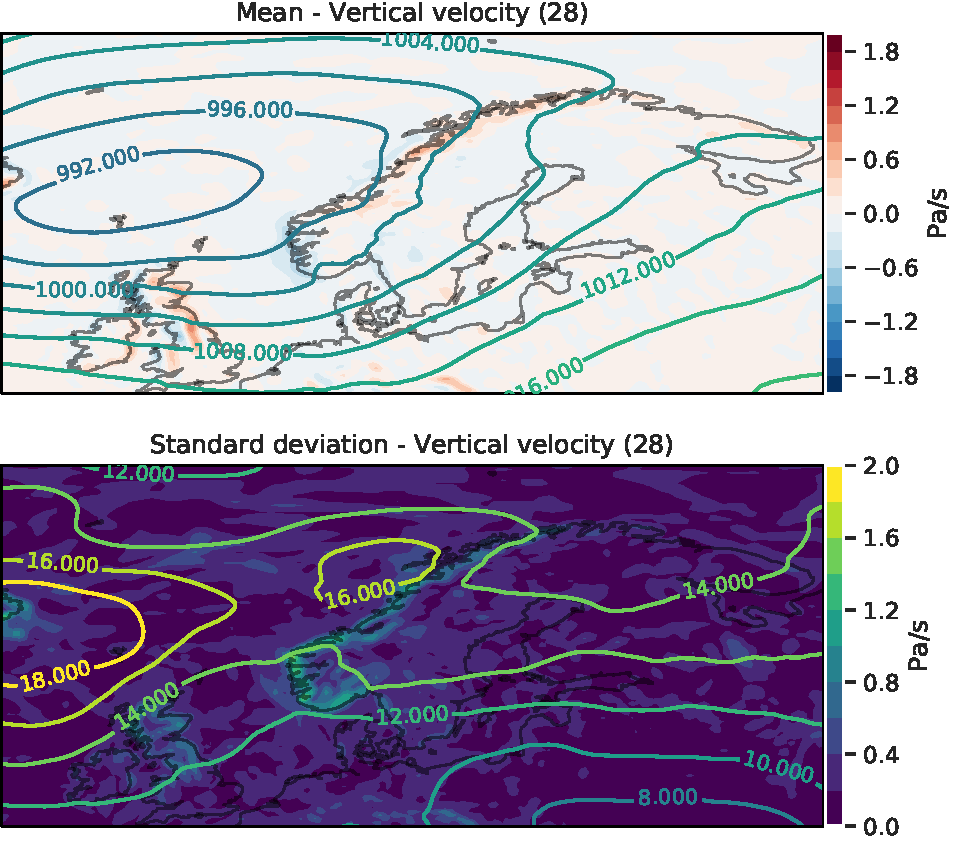
\includegraphics[width=\textwidth]{Figures/WENZV.pdf}
         \caption{Sola}
         \label{fig:ENZVW}
     \end{subfigure}
    \begin{subfigure}[b]{0.5\textwidth}
    \centering
    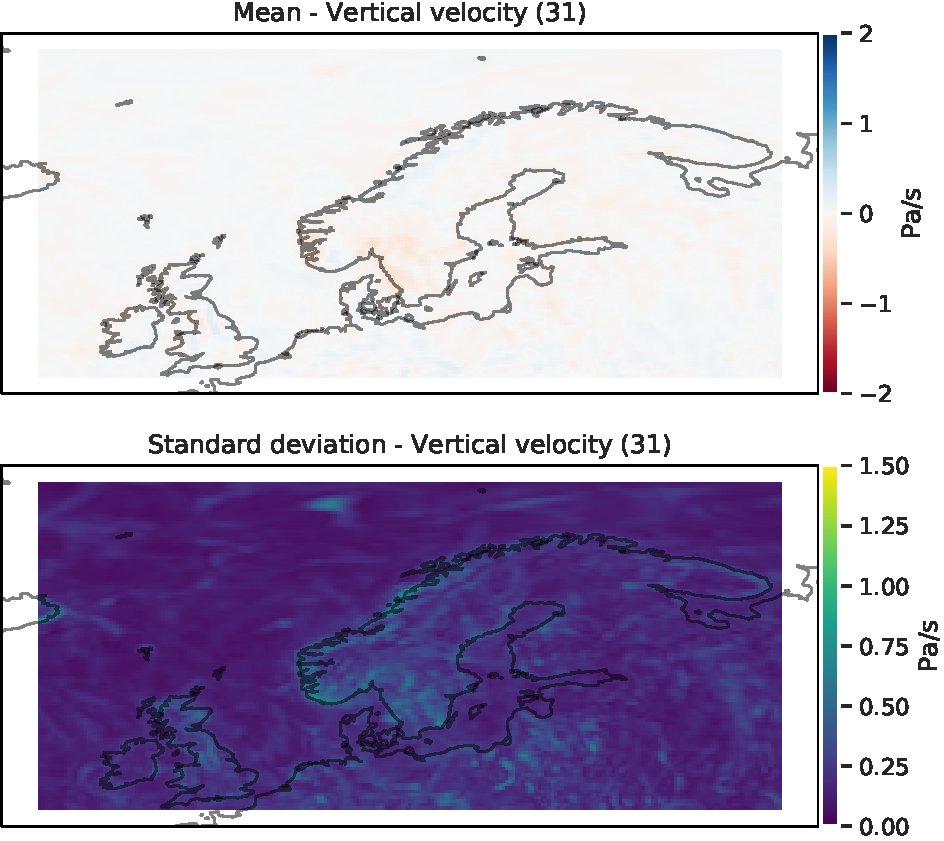
\includegraphics[width=\textwidth]{Figures/WENGM.pdf}
    \caption{Temperature for cases in Gardermoen zone.}
    \label{fig:ENGMW}
\end{subfigure}
\caption{Vertical velocity composites for the biggest airports}
\label{fig:verticalairports}
\end{figure}

\subsubsection{Large scale precipitation}
Figure \ref{fig:largescalezones} contains the large scale precipitation composites for the cases. Starting with Figure \ref{fig:NordlsP}: We see no clear pattern in the large scale precipitation for the north zones, except maybe a hint in Nordland fylke. The standard deviation also shows variation in the north region, but most of the variation is situated on the west coast. 

The picture is somewhat the same in the northwest zone in Figure \ref{fig:NordWestlsP} although here we see somewhat less precipitation in the coastal areas of the northwest zone compared to the west coast.

Figure \ref{fig:WestlsP} shows a clear pattern of precipitation for the west coast. And here also we see less variation for both Flesland and Sola, which are the most contributing airports in the dataset. 

Lastly, in Figure \ref{fig:SouthlsP}, we see that the southern coast of Norway and the northern part of Denmark have a clear contribution to the pattern here. Although some strong variation is seen in the standard deviation. Here we also see that the standard deviation is somewhat high for the whole region, hinting to that the large scale precipitation is not a good indicator for the cases in this zone.

\begin{figure}
\begin{subfigure}[b]{0.49\textwidth}
    \centering
    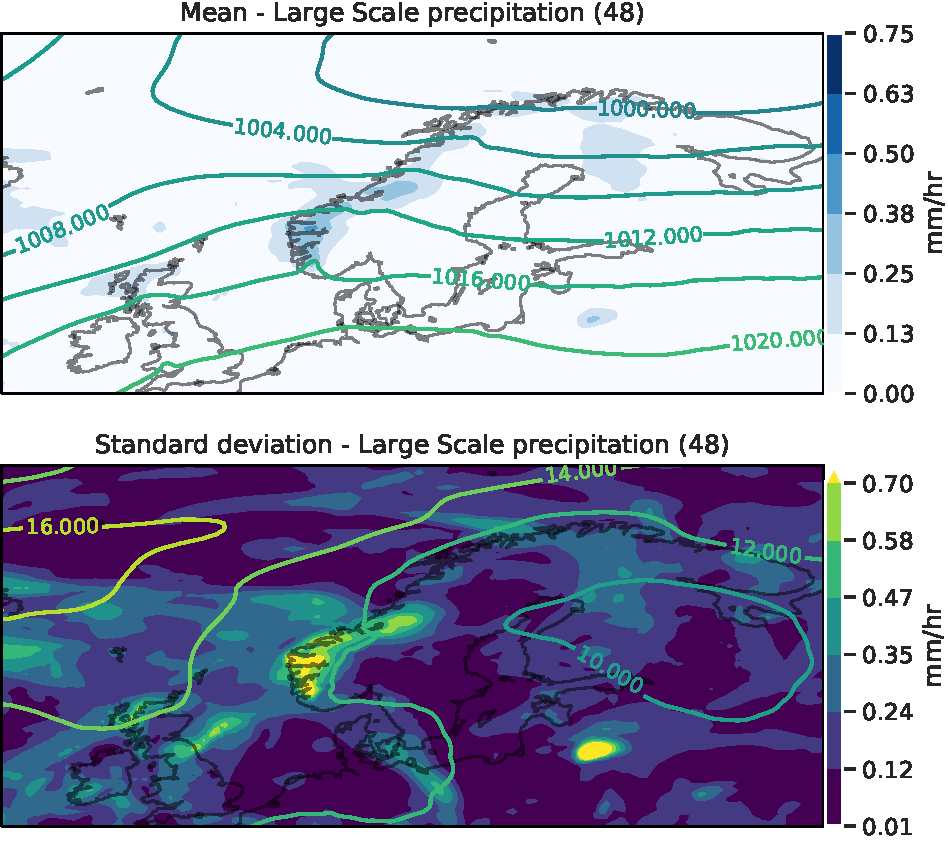
\includegraphics[width=\textwidth]{Figures/lsPNord.pdf}
    \caption{Temperature for cases in North zone.}
    \label{fig:NordlsP}
\end{subfigure}
\begin{subfigure}[b]{0.49\textwidth}
    \centering
    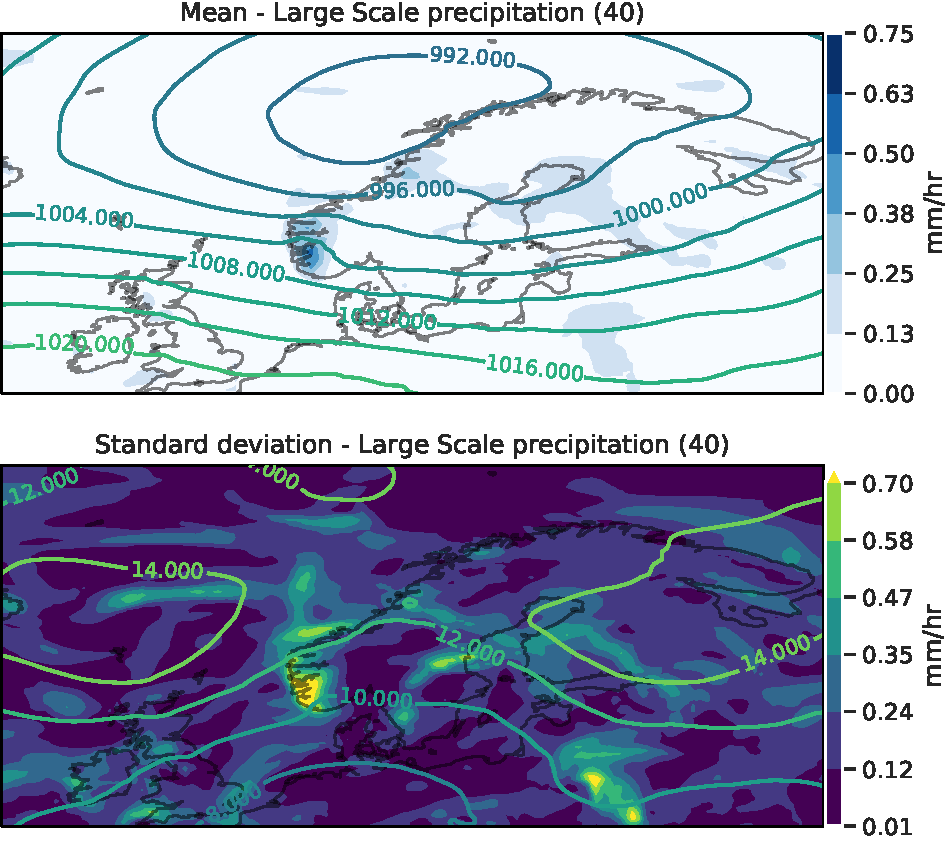
\includegraphics[width=\textwidth]{Figures/lsPNordvest.pdf}
    \caption{Large scale precipitation for cases in Northwest zone.}
    \label{fig:NordWestlsP}
\end{subfigure}
\begin{subfigure}[b]{0.49\textwidth}
    \centering
    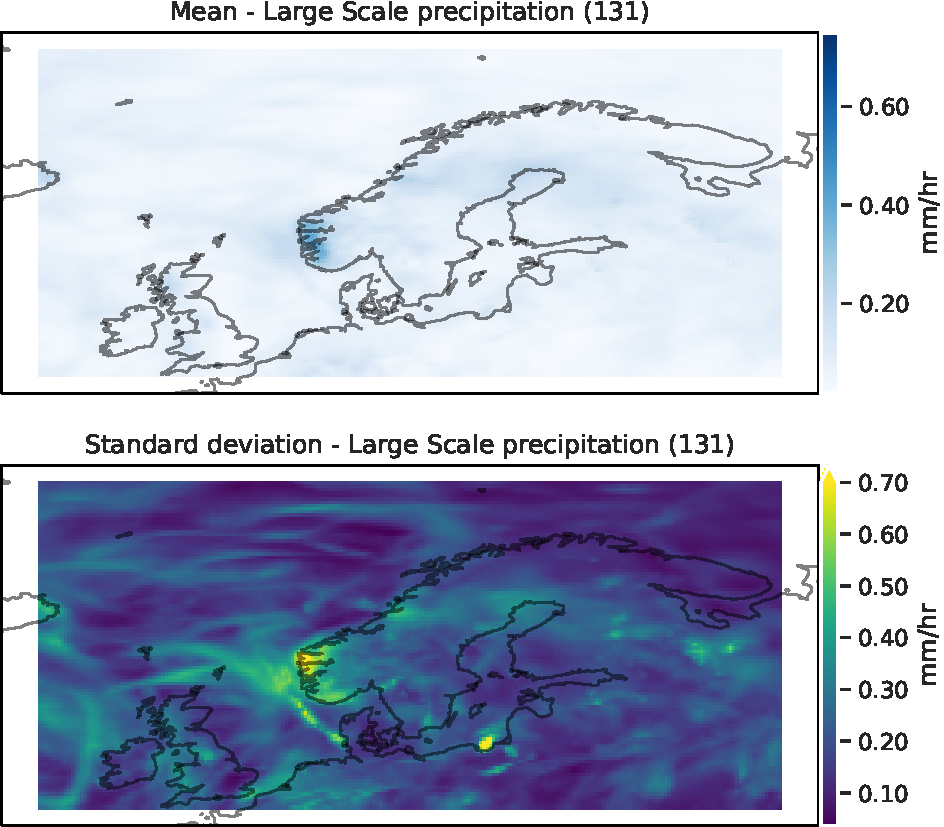
\includegraphics[width=\textwidth]{Figures/lsPVest.pdf}
    \caption{Large scale precipitation for cases in West zone.}
    \label{fig:WestlsP}
\end{subfigure}
\begin{subfigure}[b]{0.49\textwidth}
    \centering
    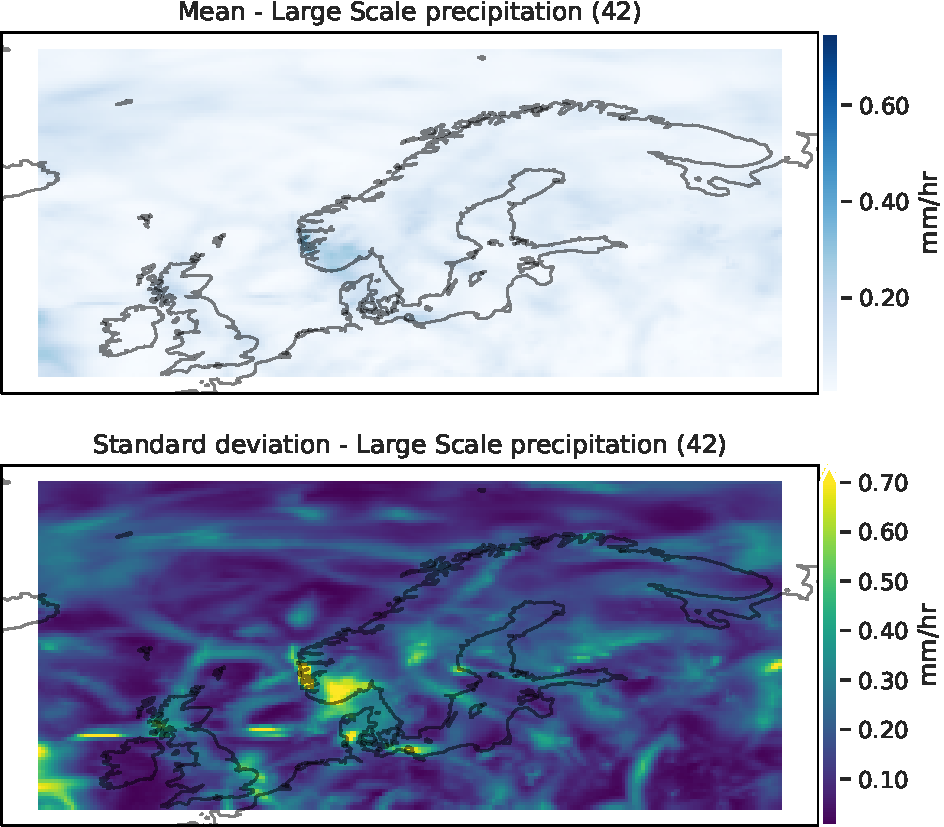
\includegraphics[width=\textwidth]{Figures/lsPSor.pdf}
    \caption{Large scale precipitation for cases in South zone.}
    \label{fig:SouthlsP}
\end{subfigure}
\caption{Large scale precipitation composites for the different zones}
\label{fig:largescalezones}
\end{figure}

In Figure \ref{fig:largescaleairports}, we see the large scale precipitation patterns divided by airports. From Figure \ref{fig:ENBRlsP} we see a pattern along the west coast of large scale precipitation. The standard deviation shows, though, a lot of variance for this area. The same is seen for Sola, in Figure \ref{fig:ENZVlsP}, and here we see a large variation. Although these patterns are shifted southwards toward Sola, and also are situated farther off the coast (above sea). For the \ref{fig:ENGMlsP} we see a weak signal around Gardermoen and eastern Norway/western Sweden. We also see that the variance is somewhat low around Gardermoen. This may hint to Gardermoen having some large scale precipitation, but not that the large scale precipitation is causal to these events. 

\begin{figure}
     \centering
     \begin{subfigure}[b]{0.49\textwidth}
         \centering
         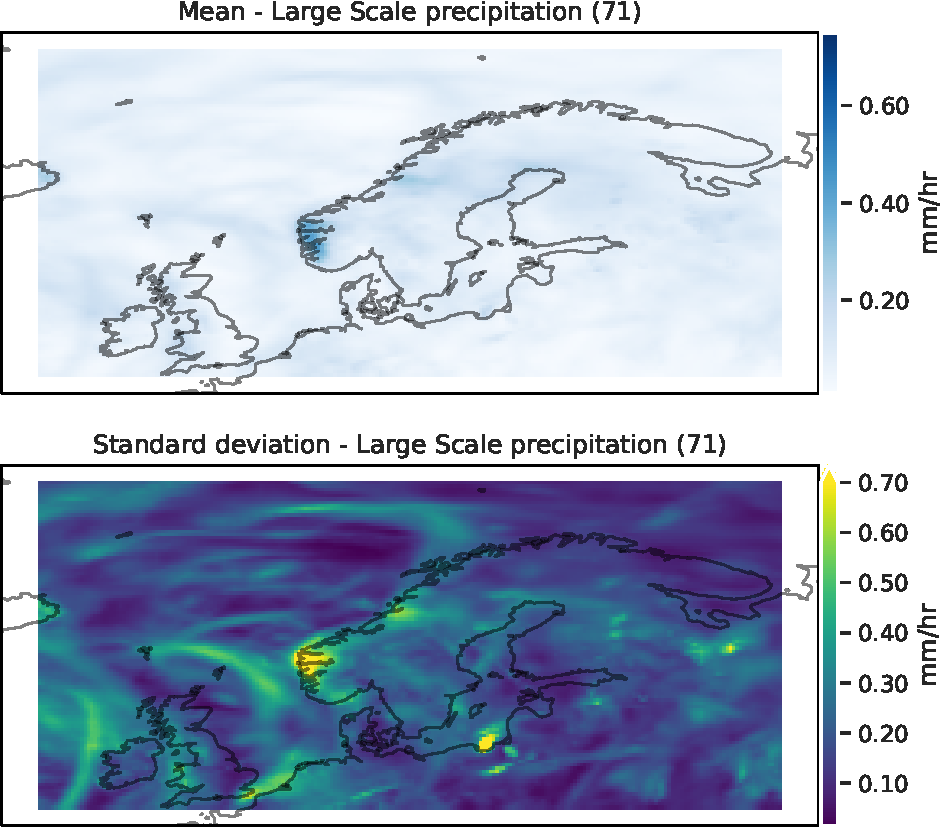
\includegraphics[width=\textwidth]{Figures/lsPENBR.pdf}
         \caption{Large scale precipitation for cases at  Flesland.}
         \label{fig:ENBRlsP}
     \end{subfigure}
     \hfill
     \begin{subfigure}[b]{0.49\textwidth}
         \centering
         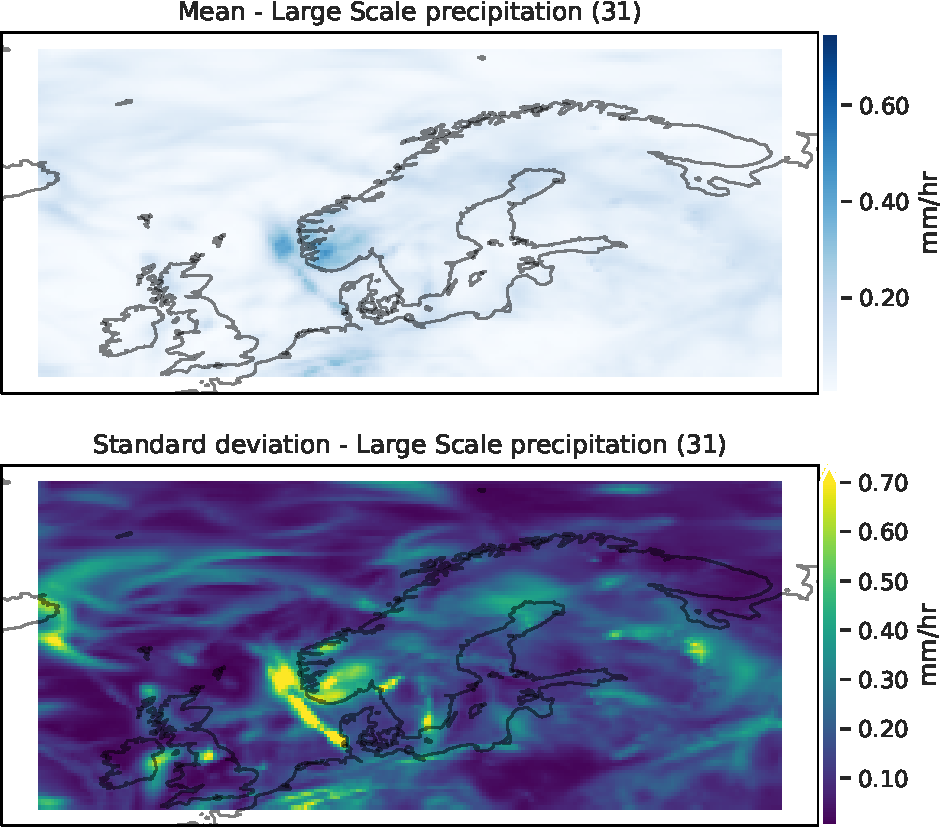
\includegraphics[width=\textwidth]{Figures/lsPENZV.pdf}
         \caption{Large scale precipitation for cases at Sola.}
         \label{fig:ENZVlsP}
     \end{subfigure}
     
    \begin{subfigure}[b]{0.5\textwidth}
    \centering
    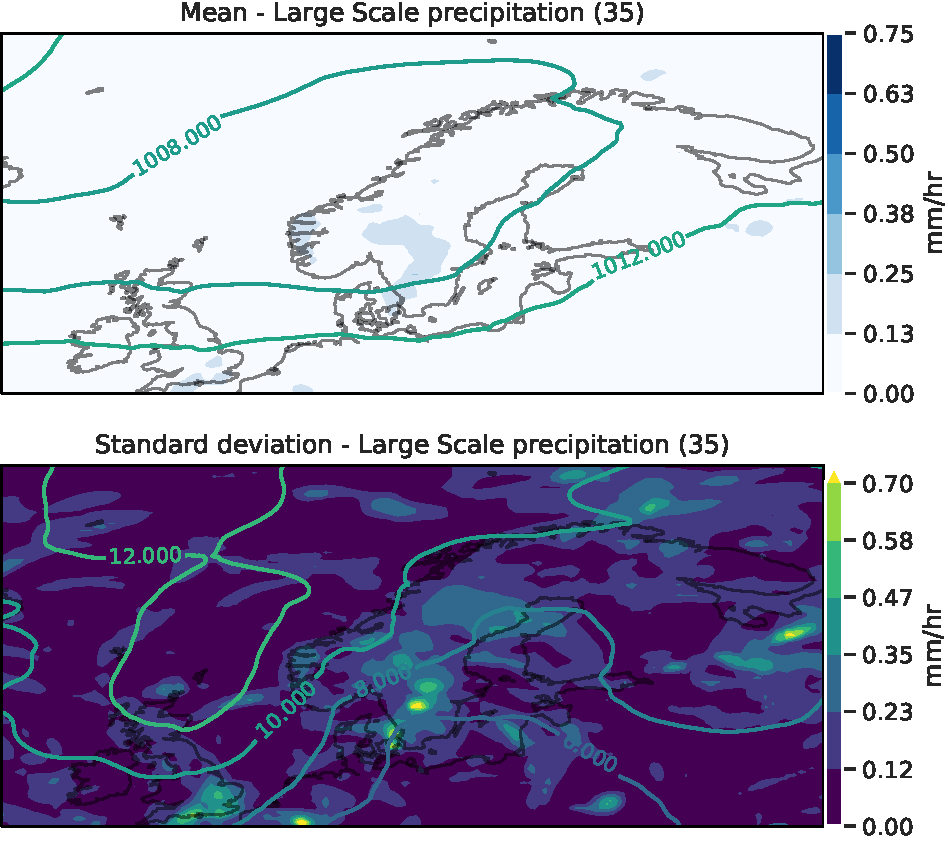
\includegraphics[width=\textwidth]{Figures/lsPENGM.pdf}
    \caption{Large scale precipitation for cases at Gardermoen.}
    \label{fig:ENGMlsP}
\end{subfigure}
\caption{Large scale precipitation composites for the biggest airports}
\label{fig:largescaleairports}
\end{figure}

\subsubsection{Convective precipitation}

Figure \ref{fig:convectivezones} shows the convective precipitation composites for the cases. In Figure \ref{fig:NordcP} we see a clear signal in the convective precipitation along the north coast. This is in contrast to the large scale precipitation we saw in Figure \ref{fig:NordlsP}. Considering the standard deviation being somewhat high hints to a problem with placing of convective systems, as discussed earlier considering the vertical velocity. This may be caused by the large geographical spread of the North zone.

Further, from Figure \ref{fig:NordWestcP} we see also a clear pattern along the northwest coast. Here, too, we have some variation in the standard deviation. 

Figure \ref{fig:WestcP} shows a very clear signal along the west coast. In fact, much stronger than the large scale precipitation (Figure \ref{fig:WestlsP}). Although here the variation is larger, this may hint at a placement problem rather than a magnitude problem. 

For the south (Figure \ref{fig:SouthcP}) we see a somewhat consistent pattern for the Norwegian and Swedish south and northern part of Denmark: Although here we see some variation in the standard deviation, and this of course may be related to the geographical spread of this zone.

\begin{figure}
\begin{subfigure}[b]{0.49\textwidth}
    \centering
    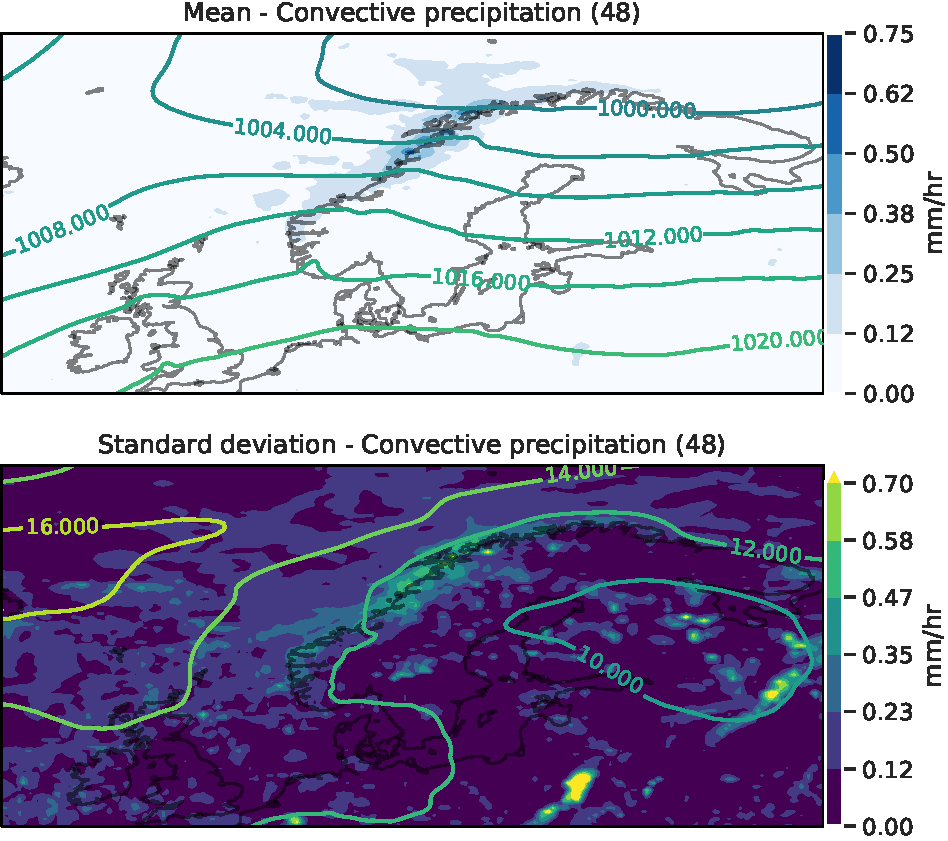
\includegraphics[width=\textwidth]{Figures/cPNord.pdf}
    \caption{Temperature for cases in North zone.}
    \label{fig:NordcP}
\end{subfigure}
\begin{subfigure}[b]{0.49\textwidth}
    \centering
    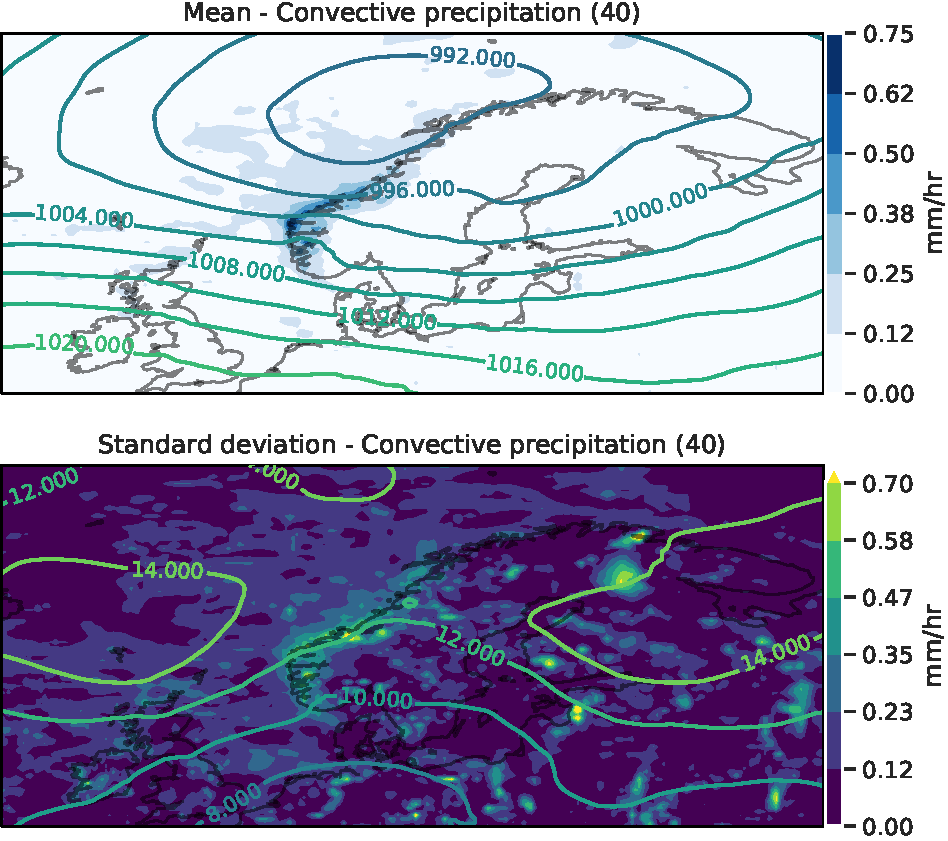
\includegraphics[width=\textwidth]{Figures/cPNordvest.pdf}
    \caption{Temperature for cases in Northwest zone.}
    \label{fig:NordWestcP}
\end{subfigure}
\begin{subfigure}[b]{0.49\textwidth}
    \centering
    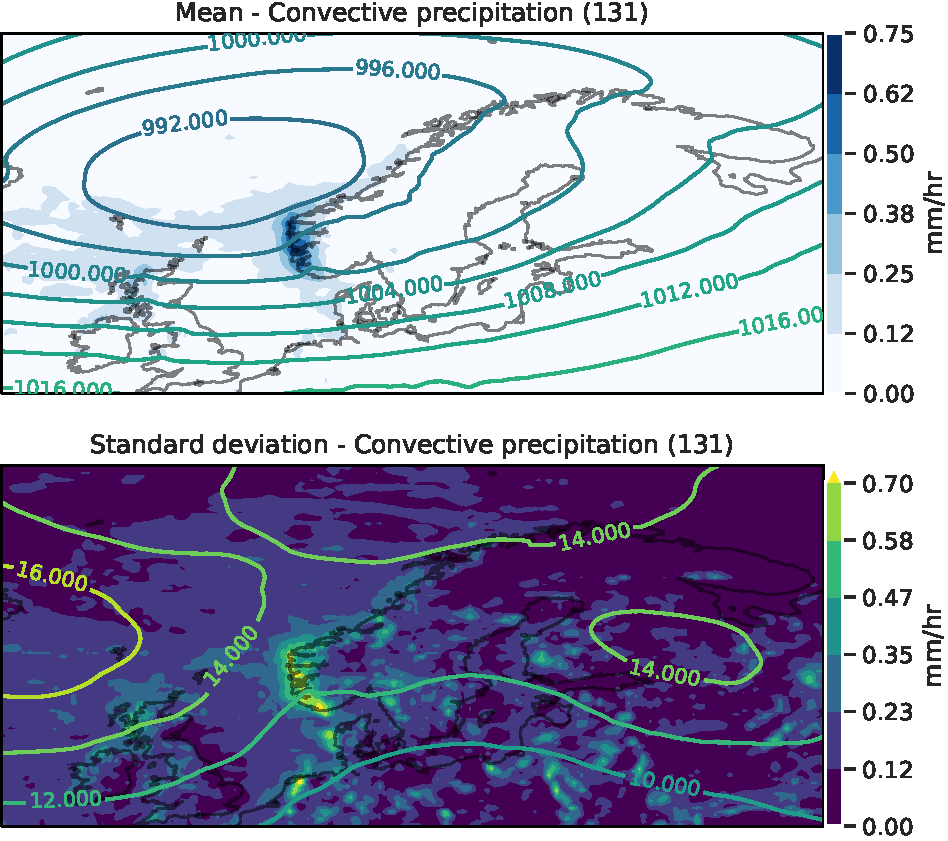
\includegraphics[width=\textwidth]{Figures/cPVest.pdf}
    \caption{Temperature for cases in West zone.}
    \label{fig:WestcP}
\end{subfigure}
\begin{subfigure}[b]{0.49\textwidth}
    \centering
    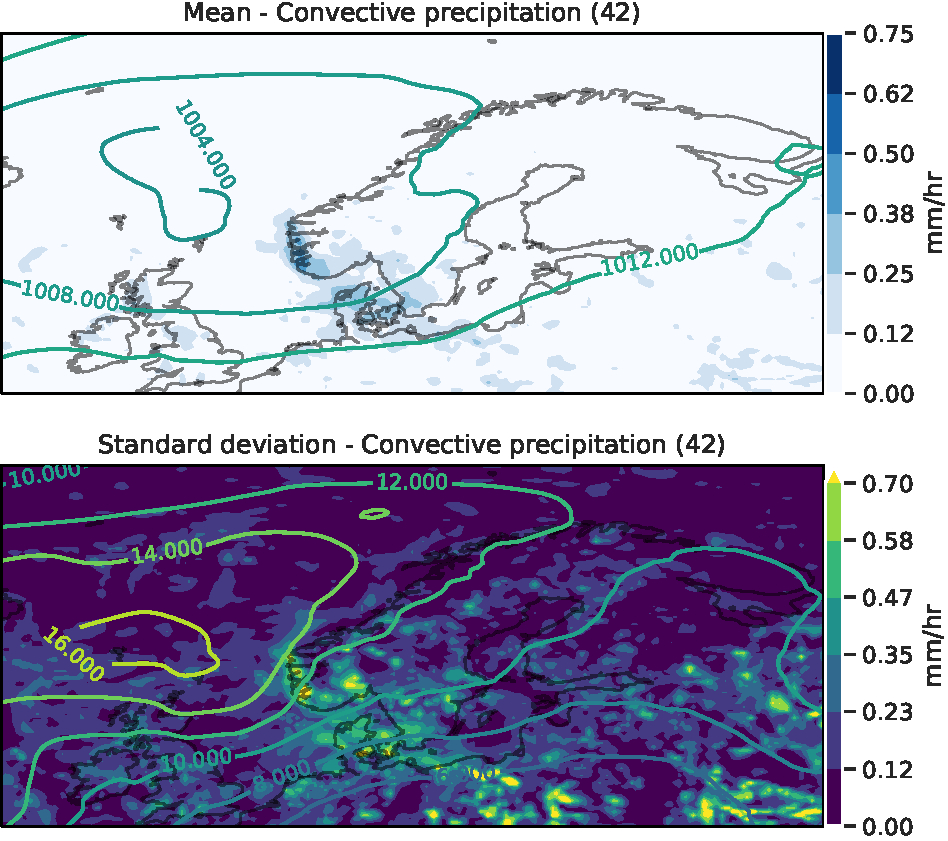
\includegraphics[width=\textwidth]{Figures/cPSor.pdf}
    \caption{Temperature for cases in South zone.}
    \label{fig:SouthcP}
\end{subfigure}
\caption{ }
\label{fig:convectivezones}
\end{figure}

Figure \ref{fig:convectiveairports} shows the composites and standard deviation of convective precipitation at the three largest airports. Figure \ref{fig:ENBRcP} shows convective precipitation being present along the west coast for most of the cases. Here we also see a much smaller standard deviation for Flesland compared to Figure \ref{fig:WestcP} such that the placement of these convective systems seem to be over Flesland. Though at Sola, as shown in Figure \ref{fig:ENZVcP}, we see a strong signal in the mean precipitation, but we also see a very large standard deviation somewhat north of Sola. This can be understood by the fact that convective systems over Sola may be so local that they are not present further north. Lastly, Figure \ref{fig:ENGMcP} shows a significant pattern of convective precipitation over Gardermoen for the cases here. We also see a lot of variation along the southern part of Norway and Sweden. This variation shows the random nature of convective cell placement. 

\begin{figure}
     \centering
     \begin{subfigure}[b]{0.49\textwidth}
         \centering
         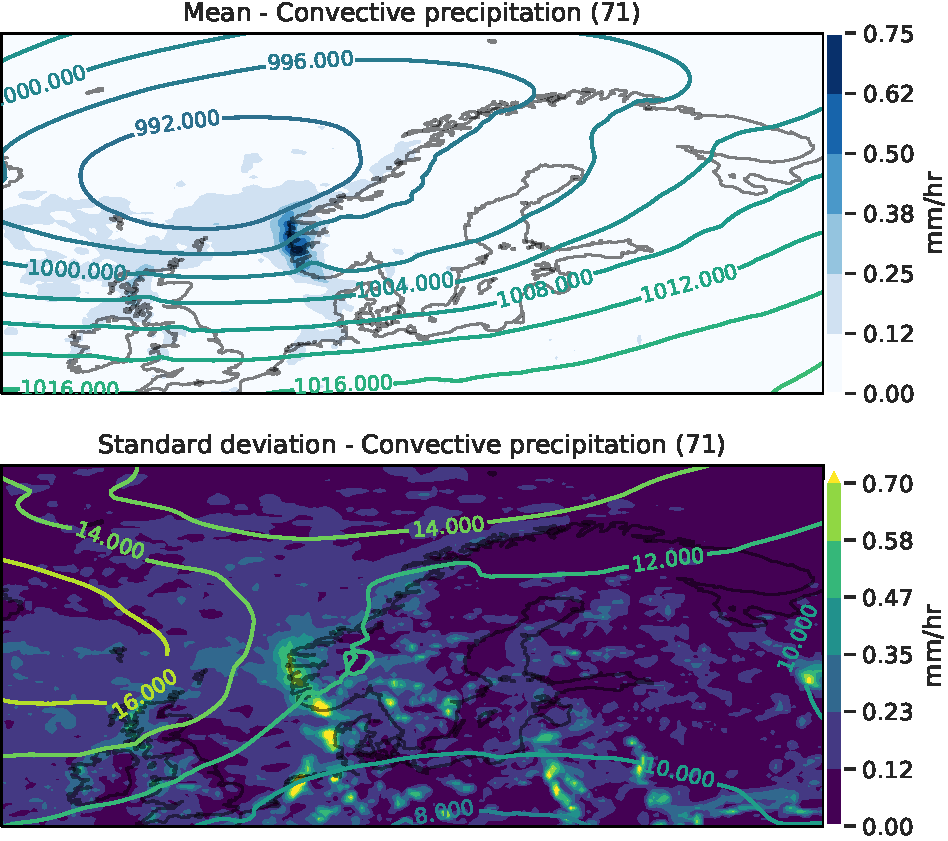
\includegraphics[width=\textwidth]{Figures/cPENBR.pdf}
         \caption{}
         \label{fig:ENBRcP}
     \end{subfigure}
     \hfill
     \begin{subfigure}[b]{0.49\textwidth}
         \centering
         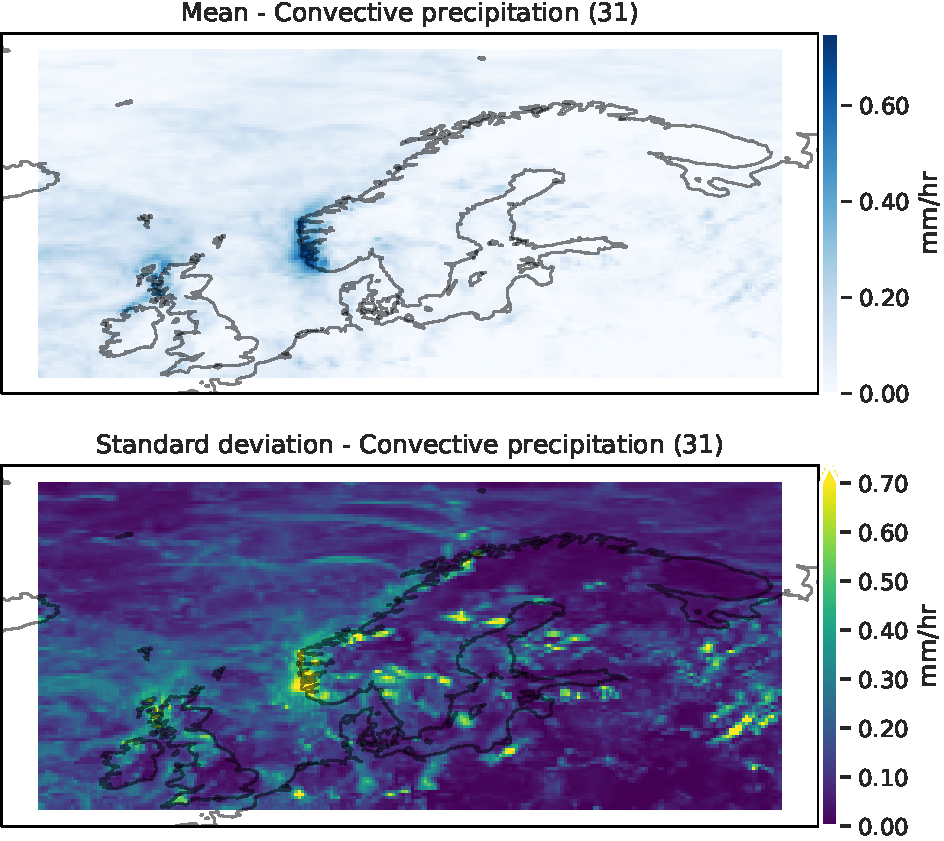
\includegraphics[width=\textwidth]{Figures/cPENZV.pdf}
         \caption{}
         \label{fig:ENZVcP}
     \end{subfigure}
     
    \begin{subfigure}[b]{0.5\textwidth}
    \centering
    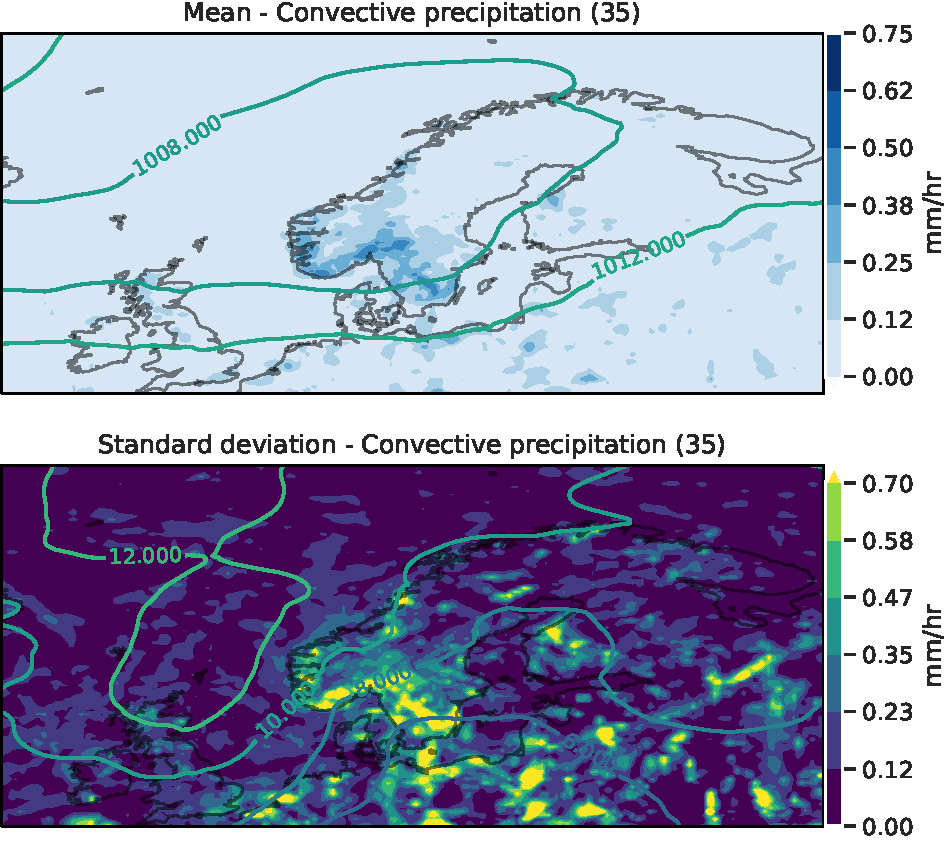
\includegraphics[width=\textwidth]{Figures/cPENGM.pdf}
    \caption{Temperature for cases in Gardermoen zone.}
    \label{fig:ENGMcP}
\end{subfigure}
\caption{ }
\label{fig:convectiveairports}
\end{figure}


\section{MEPS}
Figure \ref{fig:MeanT750MEPS} shows the same picture as discussed in section \ref{sec:era5results}: The climatological 750m temperature goes from approximately -6C to 2C along the western part of the Norwegian coast. This suggests that the mean temperature in MEPS for the HTI season is similar to the mean temperature of ERA5. If one assumes that the temperature ranges found in earlier studies, and supported in this thesis from ERA5, to be correct, one can then from this see a higher risk of \acrshort{htl} in the northern areas.

Figure \ref{fig:eramepsdiff} shows the temperature from case height for both ERA5 and MEPS. This shows a good, but varied relation between MEPS and ERA5 temperatures around and below 0C. For some cases, however, MEPS shows a significant increase in temperature compared to ERA5, e.g. six cases where ERA5 shows 0C while MEPS shows temperatures around 10C. Higher up we also see two cases in the mid-teens Celsius for ERA5, being reported 10 degrees higher for MEPS. This can be contributed to the lack of vertical resolution in the MEPS pressure levels compared to the ERA5 pressure levels. 

\begin{figure}
    \centering
    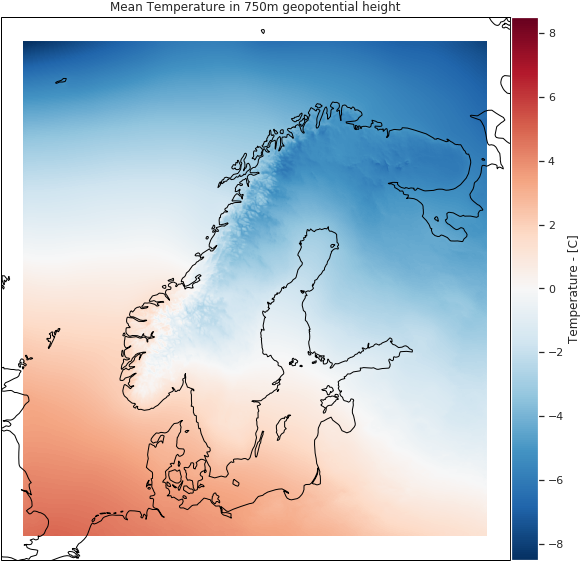
\includegraphics[width=\textwidth]{Figures/MeanT750MEPS.png}
    \caption{Mean temperature at geopotential height 750 meters for the HTI season in the control run in MEPS, with a lead time of 1-6 hours.}
    \label{fig:MeanT750MEPS}
\end{figure}

\begin{figure}
    \centering
    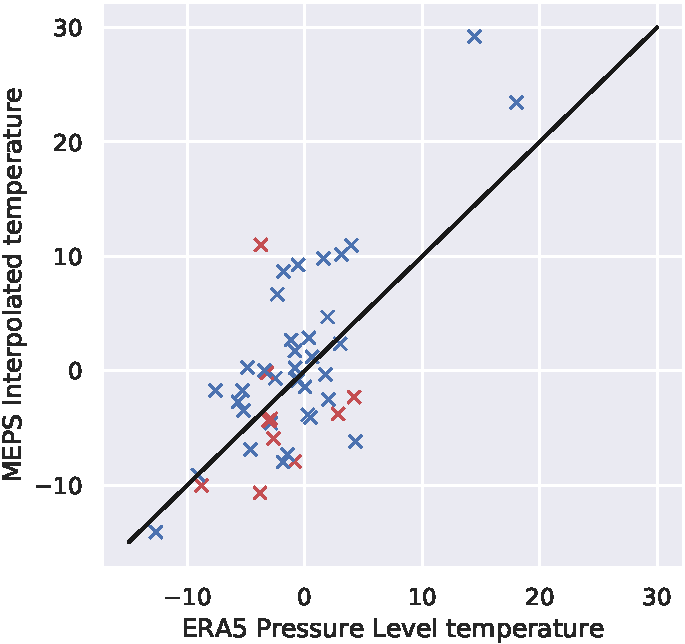
\includegraphics[width=.5\textwidth]{Figures/T750MEPSera5diff.pdf}
    \caption{difference of era5 and meps for cases}
    \label{fig:eramepsdiff}
\end{figure}

\subsection{Decomposition of HTI}

\subsubsection{Climatology}
Figure \ref{fig:temperaturemeps} shows the average value of the temperature component of the \acrshort{hti}. This shows a clear maximum signal along the northern part of Norway and a somewhat lower signal along the west coast. It should be noted that the maximum possible value in the figure is 0.25. 

\begin{figure}
    \centering
    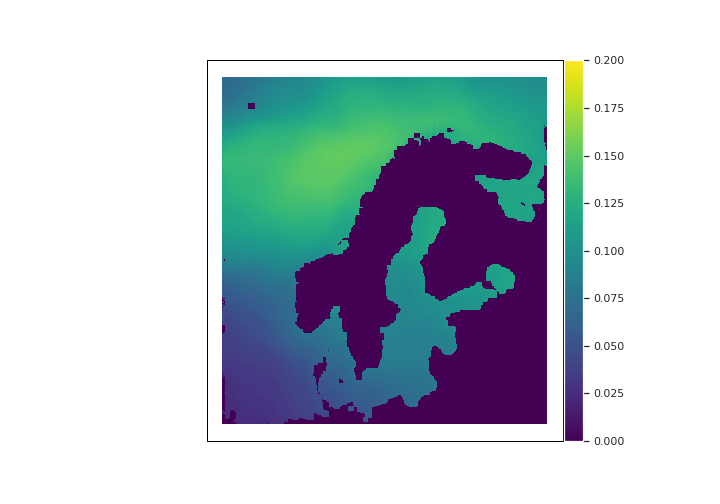
\includegraphics[width = \textwidth]{Figures/T.png}
    \caption{Temperature}
    \label{fig:temperaturemeps}
\end{figure}

Figure \ref{fig:precipitationmeps} shows the average value of the precipitation component when using accumulated precipitation instead of the intended precipitation. Here we see a strong signal off-shore and a somewhat smaller signal in the Baltic region. 

\begin{figure}
    \centering
    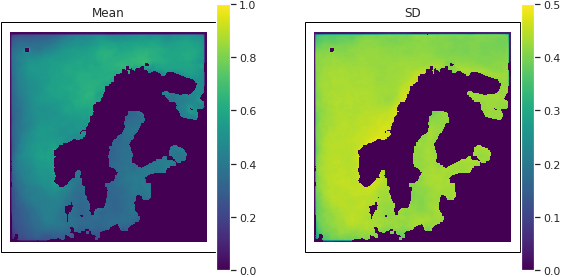
\includegraphics[width = \textwidth]{Figures/P.png}
    \caption{Precipitation}
    \label{fig:precipitationmeps}
\end{figure}

Figure \ref{fig:precipitationfixmeps} shows the substantial effects of using the intended hourly precipitation instead of the accumulated precipitation. Here we see, compared to Figure \ref{fig:precipitationmeps}, that the average value has been approximately halved.

\begin{figure}
    \centering
    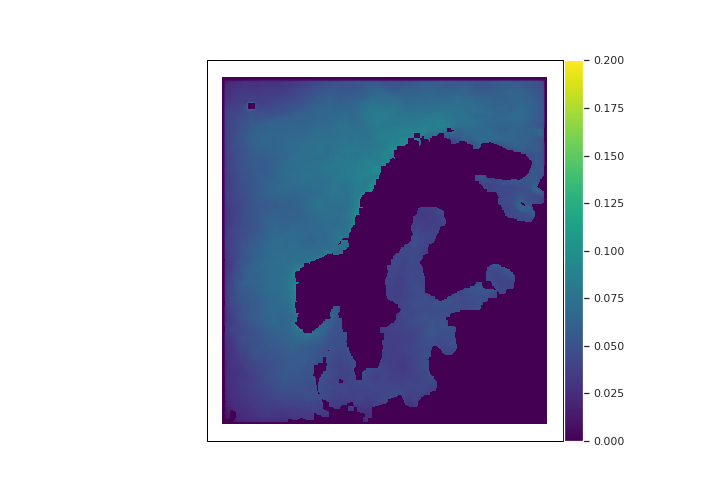
\includegraphics[width = \textwidth]{Figures/Pf.png}
    \caption{Fixed precipitation}
    \label{fig:precipitationfixmeps}
\end{figure}

Figure \ref{fig:upwardvelocitymeps} shows the average value of the vertical velocity component, and we see a strong signal along coastal parts of Norway, especially northernfacing coasts. This shows clearly the effect of the convergence approximation discussed in Section \ref{sec:hti}. Note that there is almost zero signal in the average situation over the ocean. This shows the somewhat stochasticity of convection and is also a product of the fineness of the horizontal scale. 

\begin{figure}
    \centering
    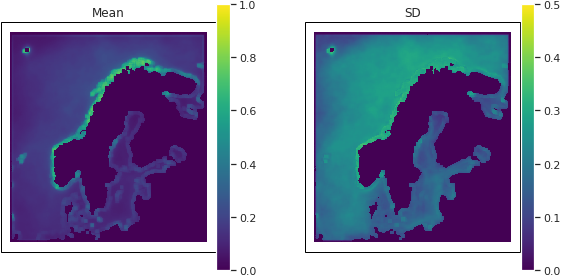
\includegraphics[width = \textwidth]{Figures/W.png}
    \caption{Vertical velocity}
    \label{fig:upwardvelocitymeps}
\end{figure}

Figure \ref{fig:cloudcovermeps} is the only of these component climatologies which is upwardly bounded. We see from the figure that off the coast of eastern Finnmark the average value is more than 0.20. (Recall that 0.25 is the maximum value of the components of the \acrshort{hti}.) In addition to this local maximum, there is also a very clear signal above the ocean, and this may be a function of the relatively high neighborhood size (7x7 cells) when calculating this parameter. 

\begin{figure}
    \centering
    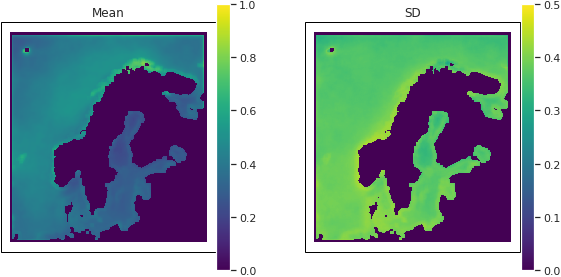
\includegraphics[width = \textwidth]{Figures/C.png}
    \caption{Cloud cover}
    \label{fig:cloudcovermeps}
\end{figure}

\subsection{Erroneous HTL-forecast}

Figure \ref{fig:fixeffect} shows the frequency of risk categories for selected airports shown in the original colors (red, orange, yellow) while the blue shade plotted over these show the frequency of risk categories \textit{after} using the hourly precipitation instead of the accumulated precipitation. This shows a reduction in the yellow category for \textit{all} airports, some showing almost a halving of yellow forecasts. Though the higher risk categories (orange and red) only show a significant reduction for the six northernfacing airports: Hammerfest, Bodø, Brønnøysund, Ørlandet, Kristiansund og Florø. Flesland and Sola do not show a reduction in the red risk, but do show a near-halving of the orange risk frequency. The equal risk in Flesland and Sola is interesting, as Flesland twice as often has incidents related to lightning as Sola.

\begin{figure}
    \centering
    \includegraphics[width=\textwidth]{Figures/climatologyyellow.png}
    \caption{Frequency of Yellow risk levels before and after fixing the erroneous forecast}
    \label{fig:fixred}
\end{figure}

\begin{figure}
    \centering
    \includegraphics[width=\textwidth]{Figures/climatologyorange.png}
    \caption{Frequency of Orange risk levels before and after fixing the erroneous forecast}
    \label{fig:fixorange}
\end{figure}

\begin{figure}
    \centering
    \includegraphics[width=\textwidth]{Figures/climatologyred.png}
    \caption{Frequency of Red risk levels before and after fixing the erroneous forecast}
    \label{fig:fixyellow}
\end{figure}

\begin{figure}
    \centering
    \includegraphics[width=\textwidth]{Figures/fixeffect.pdf}
    \caption{Frequency of [Yellow,Orange,Red] risk levels before and after fixing the erroneous forecast, for selected airports.}
    \label{fig:fixeffect}
\end{figure}

\subsection{METAR as verification}
To investigate the airports with the highest change in frequency from Figure \ref{fig:fixeffect} the observed meteorological phenomena (i.e. \acrshort{metar}) are plotted as a function of forecasted risk in both Figure \ref{fig:HTIMETAR1} and Figure \ref{fig:HTIMETAR2}. These figures show a higher frequency of meteorological observation of assumed relevant phenomena when non-white risk of \acrshort{htl} is forecast. Note that there is a slight increase in frequency of observed phenomena for the white forecasts, but there are also some decreases in frequency as the case for rain. This hints to both the increase and decrease in frequency to be not related to \acrshort{htl}. For both the red and orange risk level we see a substantial increase in observed relevant meteorological phenomena, especially showers, scattered and broken clouds, cumulonimbus and snow. Overcast and hail seem to have no considerable change, though hail may be due to the fact that it is less often reported in general.

\begin{figure}
    \centering
    \includegraphics[width=\textwidth]{Figures/HTIMetar1.pdf}
    \caption{Caption}
    \label{fig:HTIMETAR1}
\end{figure}

\begin{figure}
    \centering
    \includegraphics[width=\textwidth]{Figures/HTIMetar2.pdf}
    \caption{Caption}
    \label{fig:HTIMETAR2}
\end{figure}


\section{Suggestion for improved forecasts}

